% ======================================================================
% AAAI-27 submission format (converted from the ACL/ARR source).
% Structural/formatting changes only -- paper content is unchanged.
% The original ACL version is preserved in acl_latex.tex.
% ======================================================================

% ---- Required AAAI-27 preamble (per AuthorKit27; DO NOT CHANGE) --------
\documentclass[letterpaper]{article} % DO NOT CHANGE THIS
\usepackage[submission]{aaai2027}    % DO NOT CHANGE THIS (anonymous submission mode)
% The serif, sans-serif, and monospaced fonts are loaded automatically by
% aaai2027.sty (newtxtext, helvet, courier). Do NOT add times/helvet/courier
% or inconsolata -- they are forbidden and conflict with the style.
\usepackage[hyphens]{url}  % DO NOT CHANGE THIS
\usepackage{graphicx}      % DO NOT CHANGE THIS
\urlstyle{rm}              % DO NOT CHANGE THIS
\def\UrlFont{\rm}          % DO NOT CHANGE THIS
\usepackage{natbib}        % DO NOT CHANGE THIS (aaai2027 sets the .bst automatically)
\usepackage{caption}       % DO NOT CHANGE THIS
\frenchspacing             % DO NOT CHANGE THIS
% Keep section numbers on (2 = sections + subsections) so the paper's many
% \ref{sec:...}/\ref{apx:...} cross-references resolve. AAAI permits 0/1/2;
% never exceed 2 (subsubsection numbering breaks the style).
\setcounter{secnumdepth}{2}
\pdfinfo{
/TemplateVersion (2027.1)
}

% ---- Packages carried over from the ACL source (content-neutral) ------
\usepackage[T1]{fontenc}
\usepackage[utf8]{inputenc}
\usepackage{microtype}
\usepackage{amsmath}
\usepackage{mathtools}
\usepackage{amssymb}
\usepackage{algorithm}   % AAAI-recommended for algorithms
\usepackage{algorithmic} % AAAI-recommended for algorithms
% bbm is hard-blocked by aaai2027.sty (Type-3 fonts). Use dsfont (Type-1) and
% alias \mathbbm so any \mathbbm{...} in the source still renders identically.
\usepackage{dsfont}
\newcommand{\mathbbm}[1]{\mathds{#1}}
\usepackage{booktabs}
\usepackage[most]{tcolorbox}
\usepackage{multirow}
\usepackage{subcaption}
\usepackage{xcolor}
\definecolor{AlgGreen}{RGB}{34,139,34}

% ---- Robust asset paths (compile-root-independent) --------------------
% Figures and \input files are under latex/. These search paths let the
% document compile whether the working directory is the repo root or latex/
% (Overleaf vs. local), so nothing silently drops. \includegraphics and
% \input below are given WITHOUT the "latex/" prefix and resolved here.
\graphicspath{{latex/figs/}{figs/}}
\makeatletter
\def\input@path{{latex/}{./}}
\makeatother

% ---- Cross-reference bridge to the separate supplementary document -----
% Lets \ref{apx:...} (appendix labels, now in supplementary.tex) resolve in
% the main paper. Requires supplementary.aux to exist: compile supplementary.tex
% once, then the main paper. xr embeds no links (hyperref-free, AAAI-safe).
\usepackage{xr}
\externaldocument{supplementary}

% ---- Custom macros carried over verbatim from the ACL source ----------
% Comment macro for algorithm right-margin annotations
\newcommand{\algcmt}[1]{\hfill \textcolor{AlgGreen}{\ensuremath{\triangleright}\,#1}}

% Author annotation macros (disable/remove before submission)
\newcommand{\ml}[1]{\textcolor{orange}{\bf [lan: #1]}}
\newcommand{\mh}[1]{\textcolor{teal}{\bf [Hunter: #1]}}
\newcommand{\al}[1]{\textcolor{blue}{\bf [Alex: #1]}}

% Compact standard-deviation suffix for table cells: $0.314\std{0.016}$.
\newcommand{\std}[1]{{\scriptstyle\,\pm #1}}

\newtcolorbox{promptbox}[1]{
  colback=gray!10,
  colframe=gray!70!black,
  title=#1,
  fonttitle=\bfseries,
  arc=3mm,
  boxrule=0.8pt,
  left=6pt,
  right=6pt,
  top=6pt,
  bottom=6pt
}

\newtcolorbox{answerbox}[1]{
  colback=blue!5,
  colframe=blue!80!black,
  title=#1,
  fonttitle=\bfseries,
  arc=3mm,
  boxrule=1pt,
  left=6pt,
  right=6pt,
  top=6pt,
  bottom=6pt
}

% Qualitative counterfactual example box (appendix).
% title is braced so commas inside the title don't get parsed as pgfkeys.
\newtcolorbox{examplebox}[2][]{
  colback=gray!4,
  colframe=gray!50!black,
  title={#2},
  fonttitle=\bfseries,
  arc=2mm,
  boxrule=0.6pt,
  left=6pt,
  right=6pt,
  top=6pt,
  bottom=6pt,
  breakable,
  #1
}

% If the title and author information does not fit in the area allocated, uncomment the following
%
%\setlength\titlebox{<dim>}
%
% and set <dim> to something 5cm or larger.

% Title kept verbatim from the ACL source (already Title Case).
\title{Gumbel Machine: Counterfactual Student Writing Generation\\via Gumbel Noise Steering}

% ---- Anonymous submission author block (AAAI [submission] mode) --------
% AAAI requires "Anonymous Submission" as the sole author with empty
% affiliations for double-blind review. Restore the real author block below
% (commented) for the camera-ready version.
\author{
    Anonymous Submission
}
\affiliations{
    %
}

% ---- Real author block for camera-ready (AAAI \author/\affiliations) ---
% \author{
%     Hunter McNichols\textsuperscript{\rm 1},
%     Alexander Scarlatos\textsuperscript{\rm 1},
%     Mihai Dascalu\textsuperscript{\rm 2},
%     Danielle McNamara\textsuperscript{\rm 3},
%     Andrew Lan\textsuperscript{\rm 1}
% }
% \affiliations{
%     \textsuperscript{\rm 1}University of Massachusetts Amherst\\
%     \textsuperscript{\rm 2}University Politehnica of Bucharest\\
%     \textsuperscript{\rm 3}Arizona State University\\
%     wmcnichols@umass.edu, ajscarlatos@umass.edu, mihai.dascalu@upb.ro,
%     Danielle.McNamara@asu.edu, andrewlan@cs.umass.edu
% }

\begin{document}
\maketitle
\begin{abstract}
% 1. Motivate the problem the thing solves and provide required backgorund
An effective method of teaching across disciplines is to provide examples of high-quality work.
% This teaching method allows students to strive for an ideal in their work, and let's them take aspects of the exemplary work into their own. 
However, an example may be significantly different from a student's current work, making it challenging for them to emulate. An ideal learning demonstration is a \textit{counterfactual} version of the student work, an improved version that is still similar to their own.
% 2. Current approaches to this problem and how they fall short (the gap)
%While providing counterfactual demonstrations at scale is infeasible, advancements in large language models (LLMs) have shown considerable advances in generating counterfactual text. 
Existing automated approaches for counterfactual text generation using Large Language Models (LLMs) result in domain-specific systems that are difficult to translate into practical applications.
% which shows promise to automate but existing work is difficult to translate from laboratories and benchmarks to application-ready technology.
% 3. Present the thing (the gap fill)
We present the Gumbel Machine, a flexible, modular approach to generating counterfactuals that leverages LLM instruction-following capabilities while encouraging similarity to a reference factual text.  
% 4. Explain the thing in a sentence or two
Central to our approach is a novel, controlled decoding algorithm, $\beta$-Hindsight control, which uses latent randomness as a tunable similarity control mechanism during counterfactual generation.
% This approach can induce reference similarity and can operate in cold start settings or take advantage of task-specific training data.
% 5. Explain evidence in results
Experiments on datasets of student writing, scored on various criteria, demonstrate the effectiveness of our approach at generating counterfactuals both rubric-consistent and similar to a reference.


% Large Language Models (LLMs) have demonstrated strong capabilities for generating fluent text across a variety of tasks. A variety of data-driven techniques can be used to adapt these models to a desired task. However, while the text produced may accurately perform the task, the output is not always useful. And so on.

\end{abstract}

\section{Introduction}

% 1. Motivate counterfactual feedback as a learning tool
Providing feedback on student work, especially open-ended work, is an essential aspect of education since it helps learners identify specific areas for improvement \cite{hattie_power_2007}. There are two common ways to provide feedback: using a set of rubrics to score student work and highlight areas for improvement, and giving an example of model work. The latter faces a problem: while examples show students what exceptional work looks like, the model example might differ considerably from the student's work in terms of style, approach, or personal tendencies. This potential mismatch can make it difficult for students to see how the example can be applied to their work, thereby limiting the effectiveness of such feedback. Ideally, when receiving feedback, a student would receive a personalized, \emph{counterfactual} version of their work, which indicates small but pedagogically informative changes they can make.

%In providing feedback for complex, open-ended work, instructors often utilize rubrics that break down how student work scores across a set of criteria. In theory, any rubric-based feedback implies the existence of counterfactual work, a modified version of the graded work that would receive a different score according to the rubric. To give students an opportunity to see a counterfactual version of work, instructors may share an example work that scored highly on the rubric, demonstrating to students an ideal version of work for a given assignment. 

\begin{figure}[!t]
    \centering
    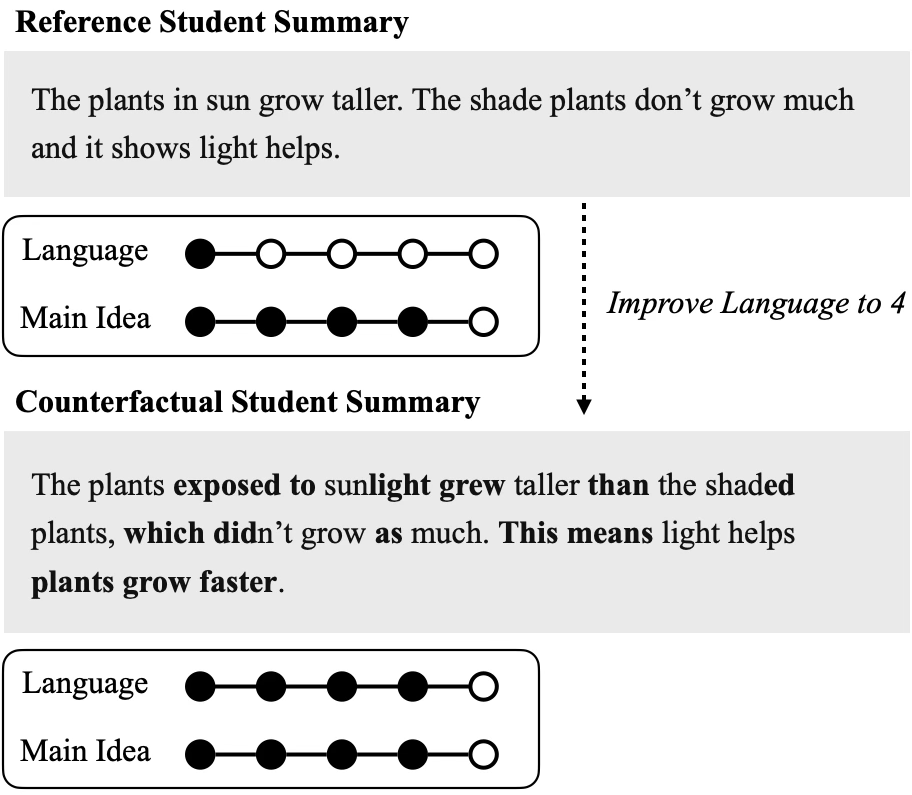
\includegraphics[width=1\linewidth]{gumbel_task_v3_2.png}
    \caption{Overview of counterfactual student writing generation. Our approach produces a revised version of student work that improves a specific rubric criterion while remaining similar to the original.}
    \label{fig:task-overview}
    \vspace{-.4cm}
\end{figure}
% \ml{good example, but the edit here is kinda substantial (more than half of the words are bolded). it also obviously uses words/language for a higher age group, so one may wonder whether that needs to be controlled as well}


% 2. Expose the difficulty in counterfactual feedback (tada llms are cool)
While personalized counterfactual student work can be pedagogically helpful, manually crafting it can be labor-intensive and hard to scale. However, when student work is textual, recent advances in natural language processing, particularly Large Language Models (LLMs), provide opportunities for automation. Recent work leverages LLMs to generate counterfactual examples for a wide range of purposes, such as story rewriting \cite{chen_unsupervised_2022}, augmenting training data \cite{qiu_paircfr_2024, zhang_dually_2025}, or enhancing model interpretability \cite{ross-etal-2021-explaining}. These findings show the promise of using LLMs to automate the generation of counterfactual student work. 



% 3. Sketch existing approaches, and gaps in existing work which motivates our contributions
Existing LLM-based approaches to automated counterfactual generation must address a central design challenge: balancing the tradeoff of task performance and similarity to the original factual text. Since these two objectives are often in opposition, a variety of approaches exist to address this tradeoff. Some approaches optimize a language model for this joint objective \cite{jung_counterfactual_2022,hu_causal_2021,dathathri_plug_2019}, thereby encoding the trade-off in its weights. Another common pattern across approaches is to decompose the problem into identification and replacement steps, where one model identifies words of the factual text that should be revised and a second replaces them for the counterfactual task. The models used in each step are either LLMs trained for the specific step on a given task \cite{ross-etal-2021-explaining,treviso_crest_2023} or a large pretrained LLMs \cite{chen_disco_2023, dixit_core_2022, sachdeva_catfood_2024, wang_fitcf_2025}. This decomposition-based approach implicitly enforces similarity by the assumption that changing only the words with maximum influence will minimize the total number of words changed, thereby enforcing similarity by construction. 

While existing approaches provide promising directions towards generating counterfactual student work, significant work remains to make them adoptable in real classrooms \cite{filighera_towards_2022}. One limitation is the tight coupling between task alignment and similarity control: many approaches rely on training task-specific classifiers or control codes, which jointly define what constitutes a valid counterfactual and how to generate them. As a result, adapting to a new task often requires retraining or system redesign, which limits generalizability. A second limitation is that most existing works frame counterfactual generation in terms of nominal labels, such as sentiment, topic, or toxicity. In these settings, success is defined by crossing a decision boundary since counterfactuals are evaluated by the resulting change in label. %This formulation obscures the notion of degree or direction of change, favoring minimal boundary-crossing edits over structured, incremental change. 
In education, however, student work is often scored in an ordinal way. Therefore, counterfactual work needs to reflect nuanced adjustments in student work that lead to continuously improved quality.
%When counterfactual generation is only designed for coarse-grained levels of correctness, the resulting feedback may be technically valid but pedagogically limited.


% Explicitly listing our contributions: outlining what we do in the rest of the paper
\textbf{Contributions} In this paper, we propose the Gumbel Machine, a modular approach for counterfactual generation that decouples similarity control from counterfactual task alignment. We first introduce $\beta$-Hindsight control, a model-agnostic, inference-time controlled decoding mechanism that recovers and reuses the stochastic state implied by a reference to induce similarity during generation. Furthermore, we detail how to combine this mechanism with a preference optimization strategy to improve an LLM's adherence to a rubric. Together, these components form our counterfactual generation approach that enables both specific control over task validity and adjustable control over similarity to a reference.
% \textbf{Contributions} In this work, we propose a modular framework for counterfactual generation that decouples similarity control from counterfactual task alignment. We first introduce $\beta$-Hindsight sampling, a model-agnostic, inference-time steering approach that recovers and reuses the stochastic state implied by a factual input to induce similarity during LLM generation. Furthermore, we demonstrate that combining this steering approach with task alignment via preference optimization results in a counterfactual generation approach that outperforms baseline prompting and steering approaches.

We evaluate our combined approach on two real-world datasets of scored student-written essay summaries using an ordinal rubric, showing flexibility beyond standard nominal evaluation settings. We show that our approach yields counterfactuals that are more similar and valid compared to multiple baselines, on both open-weight and proprietary models.
% We measure counterfactual validity with a scoring model that scores the counterfactual work under a rubric. 
In addition, we hire teachers to evaluate our approach and find that they consider our counterfactuals more similar to the original student work and, in such cases, prefer them for pedagogical use. 
% In addition, we show that $\beta$-Hindsight allows for a higher degree of control over reference similarity compared to baseline control approaches. 
Finally, we perform ablation studies on our approach to study the conditions under which the recovered stochastic state serves as an effective control signal.
% , offering insight into how instruction-following behavior and randomness interact within LLMs.
% We show that this similarity control mechanism provides a wider degree of control between task-validity and reference similarity compared to baseline, prompt-based, and controlled decoding approaches. Furthermore, we show that combining this mechanism with task alignment training via preference optimization yields an approach to generate counterfactuals that are more similar and valid than a prompting-based baseline with a much larger LLM.

% \ml{these contributions sound substantial. i hope your results can back them up}


\section{Background and Related Work}
\subsection{Gumbel-Max Trick}\label{sec:trick}

In our approach to generating counterfactual student work, we leverage the Gumbel-Max trick, which we briefly detail below. The Gumbel-Max trick is a procedure to sample from an arbitrary categorical distribution that involves adding noise sampled from a Gumbel distribution \cite{Maddison2014AS}. The samples from this procedure are shown to be equivalent to directly sampling from the categorical distribution, but the trick has the added benefit of decomposing the sampling into a reusable noise artifact that can be used to replay the randomness of the sampling process. 
% This decomposition has properties that have allowed for its use in a variety of other scenarios in machine learning, most notably in inspiring the Gumbel-Softmax procedure, which permits gradient-based optimization over categorical variables TODO cite.


\begin{figure*}[t]
    \centering
    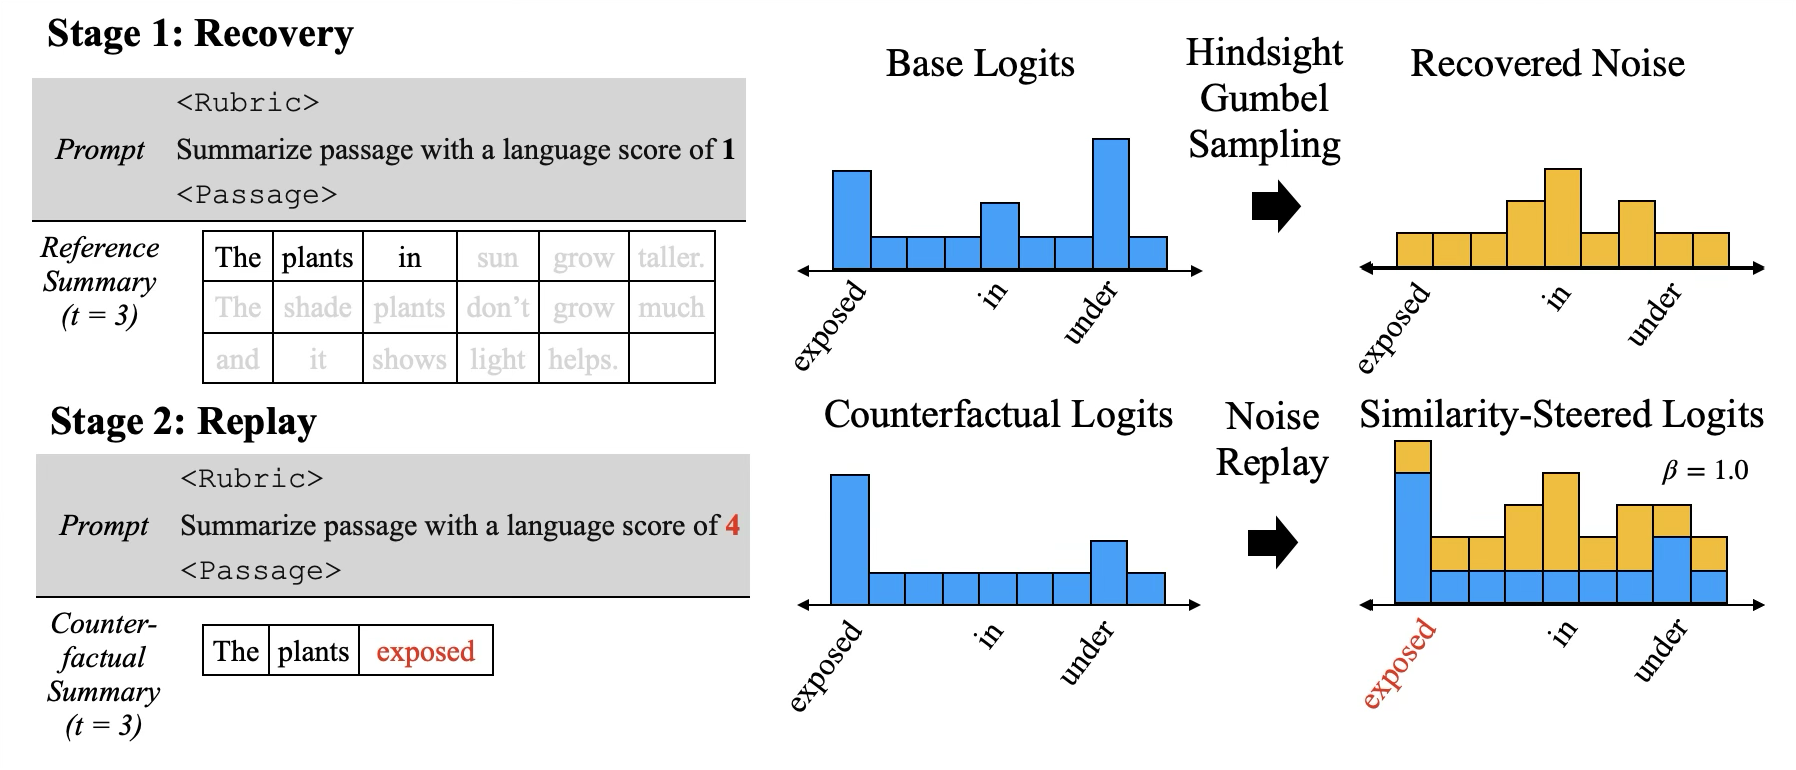
\includegraphics[width=0.95\linewidth]{gumbel_method_v2_6.png}
    \vspace{-.4cm}
    \caption{Overview of the Gumbel Machine. In Stage 1, we recover noise that would have produced the observed tokens. In Stage 2, we intervene on the prompt with a new target score and replay the noise, steering generation toward a modified score while preserving similarity to the reference. In this example, ``exposed'' is selected, while the original token ``in,'' is a close alternative. A tunable $\beta$ scales the influence of noise-based similarity on replay.}
    % i'm not 100\% sure whether this example illustrates the gist of this whole ``use-the-same-noise'' approach. the obvious: the noise didn't change what the logit (without) would likely say, which is also to generate exposed when the score is 4. the deeper: if the control is language fluency/coherence, noise contains stylistic/content things. like where the explanation goes, the logic, etc. those should be preserved. so ideally, a good counterfactual should stick to the factual summary as much as possible in terms of how the student structures things, but introduce modifications mostly in-place, fix grammatical errors, fluency issues, etc.}}
    \label{fig:method-overview}
    \vspace{-.3cm}
\end{figure*}

%We formally introduce this trick by first stating the output of an LLM, the probability of the next token, expressed in terms of the logits the model produces.
An LLM uses the softmax to sample tokens:
$$P(Y = v) = \frac{\exp(\ell_v)}{\sum_{v' \in V} \exp(\ell_{v'})}.$$
Here, $Y$ is a random variable for the next output token; $V$ is the model's vocabulary, the set of all tokens the model is trained to output; and $\ell_v$ are the \emph{logits} for each token $v \in V$. 
%In our work, we consider logits produced by transformer-based, neural language models that are conditioned on a prompt and previously generated tokens.
% This equation is a simple softmax formulation to convert the un-normalized scores into a formal probability distribution over likely next tokens.
%
Since we express $Y$ in terms of logits, we can use the Gumbel-Max trick to sample the next token instead of sampling from $P(Y)$ directly. We draw a noise sample from the Gumbel distribution for each token and add it to the logits. We then take the maximum perturbed logit index and find the corresponding token: 
% \ml{paragraphs like this one are where you can easily save space. the final line has only one or two words - you can easily find a way to rewrite the last couple sentences to shorten a bit. i fixed several places but there are a lot more}
$$ y = \arg\max_{v \in V} (\ell_v + g_v).$$
Here, $g_v \sim \text{Gumbel}(0,1)$ is an independent draw from a standard Gumbel distribution. This simple procedure is mathematically equivalent to directly sampling from $P(Y=v)$. Moreover, the Gumbel noise values can be stored to preserve the random state of the sampling process.

In our approach, we use the recovered Gumbel noise for counterfactual generation, as it enables us to keep the exogenous component of sampling fixed after applying an intervention to a language model. Concretely, we record the sampled Gumbel values, update the LLM input, and then replay the Gumbel-Max trick with the recorded ``factual'' noise values on the counterfactual logits.
% \mh{maybe last sentence can be moved/restated in intro}
% an  approach to counterfactual generation, since this noise allows us to control for randomness after applying an intervention to the model.
% We take advantage of this preservation of noise to form counterfactual outputs, since the preserved random noise can be used to control exogenous variables of the language modeling stochastic process and allow for analysis of the effect of various model interventions.


\subsection{Hindsight Gumbel Sampling}

The Gumbel-Max trick provides a mechanism for preserving and replaying the random noise used in discrete random processes. However, in practice, we often do not have access to the random process and can only observe samples. For example, the random process that generates student writing is controlled by the students themselves, not a computational system that produces logits. Therefore, we need to approximate the random process and recover the noise implied by the observations. \citet{ravfogel2025gumbel} refers to the task of recovering noise from a proxy as ``Hindsight Gumbel Sampling.'' In their work, the authors use an LLM as a proxy for the textual data generation process and outline an algorithmic procedure to recover Gumbel noise implied by data. We build on this foundation and demonstrate that recovered noise can serve as a tunable similarity-control mechanism. 

\subsection{Related Work}

\paragraph{Counterfactual Generation.} Counterfactual text generation has been widely studied, within NLP, for applications for a variety of tasks including sentiment analysis~\cite{kaushik_learning_2020, madaan_generate_2021}, story rewriting~\cite{chen_unsupervised_2022}, question answering~\cite{sachdeva_catfood_2024, paranjape_retrieval-guided_2022}, relation extraction~\cite{miao_episodic_2024}, and domain adaptation~\cite{calderon_docogen_2022, wu_polyjuice_2021}. Recent work has also explored applications of LLMs for counterfactual generation, particularly for data augmentation and model explainability \cite{goethals_what_2025, zhang_dually_2025,wang_fitcf_2025,gat_faithful_2023, wen_autocad_2022}.

\paragraph{Counterfactuals in Education.} Extensive work has been done in education to provide feedback for short answer writing~\cite{filighera_your_2022, mcnichols_can_2024, scarlatos_improving_2024}. Closely related to counterfactual generation is the task of paraphrase generation ~\cite{ouahrani_paraphrase_2024}, but existing work on counterfactual generation remains limited, highlighting the need for further development in this domain.  

% Existing work evaluates the counterfactual reasoning capabilities of LLMs in education~\cite{sonkar_malalgoqa_2024}, but 


% \textbf{Controlled Decoding}
% \textbf{Contrastive Decoding?}

\paragraph{Gumbel Noise for LLM Generation.} Recent work has explored the use of Gumbel noise for consistency during LLM generation \cite{de_mijolla_waste_2025}. Subsequent work explores the application of Gumbel noise to counterfactual generation for analyzing language model bias \cite{chatzi2025counterfactual}. \citet{ravfogel2025gumbel} introduces a procedure for reference-based recovery and replay of Gumbel noise for counterfactual generation. 

Our approach builds on this line of work and introduces several key innovations. First, this work demonstrates that the recovered Gumbel Noise can serve as a tunable reference-similarity control signal during generation time. Second, our work is the first to extensively evaluate the quality of the Gumbel noise-generated counterfactuals for an applied downstream task. Finally, we introduce a practical variant of hindsight Gumbel sampling that does not require computing the normalization constant. 

% Our empirical findings suggest that recovered noise can only be used effectively under specific conditions, namely those where the model is provided specific instructions that hint at the required output. 
% \mh{This last bit might belong in intro/related work instead}

% Related work by \cite{chatzi2025counterfactual} uses a similar procedure to generate factual, counterfactual pairs with Gumbel noise but does not recover the noise from data

% Recent work have explored the use of Gumbel noise sampling to analyze model bias \cite{chatzi2025counterfactual} or the effect of various steering techniques \cite{ravfogel2025gumbel}. These works follow a three phase procedure towards using noise for counterfactual generation: recovery, intervention, and replay. First Gumbel noise from a ``factual'' text is recovered through an algorithmic procedure on the base, untreated language model. Second, an intervention is applied to language model such as prompt adjustment or steering. Finally, the stored noise is used to sample from treated model via the Gumbel-Max trick. While both works provide theoretical grounding in justifying their work, empirical validation is limited in scope and focus on explaining model behavior instead of leveraging recovered noise for a downstream task.

% In this work, we introduce a practical variant of the recovery procedure outlined by \cite{ravfogel2025gumbel} that allows for efficient, posterior noise recovery from ground truth reference text.  We demonstrate in this work that in order to reuse Gumbel noise on a challenging but practical task, student contrastive example generation, significant hinting is required in order for the recovered noise to meaningfully change the model. We further show that the noise that emerges from this signal can also be used to sample from the model in a meaningful way.

\section{Methodology}
In this section, we formalize the task of counterfactual generation and our approach to this task. 
% \al{For the following, we might want to approach our task from a more generic perspective, so that people doing CG for other domains feel like this applies to them. Essentially, I think we can drop the ``feedback'' term for the most part in this section, and then re-introduce it in the experiments section.}

\subsection{Counterfactual Generation Task}
In our setting, we treat both factual and counterfactual outputs as token sequences generated by an LLM in response to an instruction prompt. Formally, we assume a pretrained autoregressive LLM $f_{\mathbf{\theta}}: \mathbf{x} \rightarrow \mathbf{y}$, parameterized by weights $\mathbf{\theta}$. We define $\mathbf{x}={( x_1 \dots x_N)}$ as a sequence of tokens forming the instruction (prompt) to the model, and $\mathbf{y}={( y_1 \dots y_M)}$ as the output tokens sampled from the model. We define a counterfactual as an alternative output $f(\mathbf{x'})_{\mathbf{\theta}}=\mathbf{y}'$ obtained after an intervention to the input prompt $\mathbf{x}'$. 

In counterfactual generation, our goal is to create an output that reflects a category change intervention in the input while remaining similar to a factual reference. Formally, given a reference $\mathbf{y}_r$ in category $z$, we need to output $\mathbf{y}'$ in target category $z'$, where $z \neq z' \in \{0,\dots ,k\}$ for a task with $k$ distinct categories. 
% We define the optimal output as $\mathbf{y}^*_c$, the counterfactual which achieves the desired category $z'$ with maximum similarity to $\mathbf{y}_r$. \ml{is there a need to define this optimal output? i don't see the notation (or even the concept) reused below}
In tasks such as counterfactual topic generation, $z$ is interpreted as a nominal label, but in our counterfactual student work generation task, we interpret $z$ as an ordinal score. To determine a category for an arbitrary output, we introduce a scoring model $s: \mathbf{y} \rightarrow \hat{z}$ to estimate a score for an arbitrary output, and we say a counterfactual is \emph{valid} when $s(\mathbf{y}')=z'$.

% Finally, to evaluate an approach for this task, we need a way to determine a category for an arbitrary output. We introduce a scoring model $s: \mathbf{y} \rightarrow \hat{z}$ to estimate a score for an arbitrary output, and we say a counterfactual is valid when $s(\mathbf{y}')=z'$.

% Given a factual output $\mathbf{y}*$ with score $\mathbf{z}$, our task is to produce outputs $\mathbf{y}^*_c$ that would receive an alternative target score $\mathbf{z'}$. \al{You can be a bit more generic here, since in the CG literature people care about producing an output with respect to a target ``label''. So you can introduce $z$ as a label first, and then say in our setting this corresponds to a score, but in other domains could be something else.} 


% Thus, our objective is to generate counterfactual outputs $\mathbf{y}^*_c$ such that $s(\mathbf{y'})=\mathbf{z}'$ while remaining lexically similar to the original factual output $\mathbf{y}^*$. \al{This last sentence kind of comes out of nowhere. I think it might make sense to introduce our ``objective'' in plain English in the first sentence of this subsection, along with some quick motivation for why that is our task. Then, once we've established all the math notation, we can formalize it like you do here.}

% assume a dataset of scored factual output tuples $(\mathbf{y}^*, \mathbf{z})$. 

% , which can be as simple as a prompt adjustment $\mathbf{x}'$ or more involved such as changing the weights of the model through training and preference alignment.
%  We posit that any factual output is possible, however unlikely, under the model given a reasonable instruction prompt $\mathbf{x}$. 

% For the counterfactual feedback task, we produce a specific subset of counterfactual outputs $\mathbf{y}^*_c$ that would receive a different score while maintaining minimal distance from the factual output $\mathbf{y}^*$.

% For our interventions, we consider both adjustments to the prompt, as simple as a single character adjustment in the instructions from $z$ to $z'$, and scenarios where the model weights have changed through training and alignment.

% In our framework we view a student answer to a short answer question as a random sequence of tokens drawn from a Large Language Model (LLM). Under this framework, each student answer is viewed as a particular realization from the probabilistic output space of the LLM, conditioned on the problem prompt and any relevant context.

% We posit that a student work to a given problem can be expressed as a random sequence of tokens drawn from $f$. Under this framework, each student answer is viewed as a particular realization from the probabilistic output space of the LLM, conditioned on the input $x$.
% We further breakdown $\mathbf{x}$ which includes 1. task instructions and a rubric defining what each value of criteria is required and instructions to produce an output with a desired score $z'$ the value for the particular criteria.



\subsection{$\beta$-Hindsight Similarity Control}

% and recover the random state $\mathbf{g}$ of the model which would result in the factual output.

We now detail our inference-time similarity control approach for counterfactual generation, outlined in Algorithm~\ref{alg:gumbel-cf-short}. There are two phases: recovering the noise under a base LLM and replaying the noise values to sample from an intervened LLM.

To recover the Gumbel noise that corresponds to each token of a reference, for each autoregressive timestep $t$, we derive a noise vector $\mathbf{g}_t \in \mathbb{R}^V$ that satisfies the condition: \begin{equation} \label{max-condition}
    % \ell_{y_t} + g_{y_t} > \ell_v + g_v\  \forall v \in V, v \ne y_t
    \ell[{y_t}] + \mathbf{g}_t[{y_t}] > \ell[v] + \mathbf{g}_t[v]\  \forall v \in V, v \ne y_t.
\end{equation}
Here, $V$ is the LLM's vocabulary, $y_t$ indexes the factual reference token at timestep $t$, and $\ell[{y_t}]$ is the associated logit. We omit the subscript $r$ of the reference $y_r$ for clarity in time-based indexing. This condition ensures that the observed factual token $y_t$ is selected during the Gumbel-Max prediction.

In order to satisfy Equation~\ref{max-condition}, we form a noise vector by first sampling the target noise from a lower-truncated Gumbel distribution. 
$$
\mathrm{LowerTruncG}(\tau_{min}) \coloneqq P\bigl(G \mid G > \tau_{min}\bigr).
$$ 
Here, $\tau_{min}$ denotes the lower bound of a truncated standard Gumbel distribution. We then compute $\tau_{min} = \ell_{max} - \ell[{y_t}]$, the difference between the ground truth token logit and the maximum observed logit, so that the augmented logit for the reference token will be greater than the logit for any other token at each timestep.

% \begin{algorithm}[t]
\caption{$\beta$-Hindsight Control}
\label{alg:gumbel-cf-short}
\begin{algorithmic}[1]

\STATE \textbf{def} BetaHindsight$(\mathbf x, \mathbf y, \mathbf x', \theta, \beta)$:
\STATE \quad $\mathbf G \gets \varnothing$

\STATE \quad \textbf{for} $t = 1,\dots,|\mathbf y|$:
\STATE \qquad $\ell \gets \mathrm{LLM}(\mathbf x, \mathbf y_{<t};\theta)$
\STATE \qquad $\ell_{max} \gets \max_{v\in V} \ell_v$
\STATE \qquad $g_t(y_t) \sim \mathrm{LowerTruncG}(\ell_{max} - \ell_{y_t})$
\STATE \qquad $T_t \gets \ell_{y_t} + g_t(y_t)$
\STATE \qquad \textbf{for} $v \in V \setminus \{y_t\}$:
\STATE \qquad\quad $g_t(v) \sim \mathrm{UpperTruncG}(T_t - \ell_v)$
\STATE \qquad store $\mathbf g_t$ in $\mathbf G$

\STATE \quad $\mathbf y_c \gets \varnothing$
\STATE \quad $y'_1 \gets \mathrm{BOS},\; t \gets 1$

\STATE \quad \textbf{while} $y'_t \neq \mathrm{EOS}$:
\STATE \qquad $\ell \gets \mathrm{LLM}(\mathbf x', \mathbf y_{c_{<t}}; \theta)$
\STATE \qquad \textbf{if} $t \le |\mathbf y|$:
\STATE \qquad\quad $\mathbf g_t \gets \mathbf G[t]$
\STATE \qquad\quad $y'_t \gets \arg\max_{v\in V}\bigl(\ell_v + \beta g_t(v)\bigr)$
\STATE \qquad \textbf{else}:
\STATE \qquad\quad $u_t(v) \sim \mathrm{Gumbel}(0,1)$
\STATE \qquad\quad $y'_t \gets \arg\max_{v\in V}\bigl(\ell_v + u_t(v)\bigr)$
\STATE \qquad append $y'_t$ to $\mathbf y_c$, $t \gets t+1$

\STATE \quad \textbf{return} $\mathbf y_c$

\end{algorithmic}
\end{algorithm}
\begin{algorithm}[t]
\caption{$\beta$-Hindsight Control}
\label{alg:gumbel-cf-short}
\begin{algorithmic}[1]

\STATE \textbf{def} BetaHindsight$(\mathbf x, \mathbf y, \mathbf x', \theta, \beta)$:
\STATE \quad $\mathbf G \gets \varnothing$

\STATE \quad \textbf{for} $t = 1,\dots,|\mathbf y|$: \algcmt{Recover Noise}
\STATE \qquad $\ell \gets \mathrm{LLM}(\mathbf x, \mathbf y_{<t};\theta)$
\STATE \qquad $\ell_{max} \gets \max_{v\in V} \ell[v]$
\STATE \qquad $\mathbf g_t[y_t] \sim \mathrm{LowerTruncG}(\ell_{max} - \ell[y_t])$
\STATE \qquad $T_t \gets \ell[y_t] + \mathbf g_t[y_t]$
\STATE \qquad \textbf{for} $v \in V \setminus \{y_t\}$:
\STATE \qquad\quad $\mathbf g_t[v] \sim \mathrm{UpperTruncG}(T_t - \ell[v])$
\STATE \qquad store $\mathbf g_t$ in $\mathbf G$

\STATE \quad $\mathbf y' \gets \varnothing$
\STATE \quad $y'_1 \gets \mathrm{BOS},\; t \gets 1$

\STATE \quad \textbf{while} $y'_t \neq \mathrm{EOS}$: \algcmt{Replay noise}
\STATE \qquad $\ell \gets \mathrm{LLM}(\mathbf x', \mathbf y'_{<t}; \theta)$
\STATE \qquad \textbf{if} $t \le |\mathbf y|$:
\STATE \qquad\quad $\mathbf g_t \gets \mathbf G[t]$
\STATE \qquad\quad $y'_t \gets \arg\max_{v\in V}\bigl(\ell[v] + \beta \cdot \mathbf g_t[v]\bigr)$
\STATE \qquad \textbf{else}:
\STATE \qquad\quad $\mathbf u_t \sim \mathrm{Gumbel}(0,1)^{|V|}$
\STATE \qquad\quad $y'_t \gets \arg\max_{v\in V}\bigl(\ell[v] + \mathbf u_t[v]\bigr)$
\STATE \qquad append $y'_t$ to $\mathbf y'$, $t \gets t+1$

\STATE \quad \textbf{return} $\mathbf y'$

\end{algorithmic}
\end{algorithm}

The sampled target noise establishes a ceiling, $T_{t} = \ell[{y_t}] + g[y_t]$, the new logit value for the reference token. Subsequently, for all other tokens $v \neq y_t$, we sample their corresponding noise values from an upper-truncated Gumbel distribution, such that no resulting token logit exceeds the ceiling. 
$$
\mathrm{UpperTruncG}(\tau_{max}) \coloneqq P\bigl(G \mid G < \tau_{max}\bigr).
$$ 
Here, $\tau_{max}$ denotes the upper bound of a truncated standard Gumbel distribution. We compute $\tau_{max} = T_t - \ell[v]$, the difference between the ceiling logit value and the actual logit value, for each of the other tokens in the vocabulary, so that none of the resulting logit values would exceed the ceiling. To efficiently sample from the truncated Gumbel distributions, we perform inverse transform sampling \cite{devroye1986non}, mapping the uniform samples to the truncated support range before applying the inverse CDF. The recovered Gumbel noise values satisfy (\ref{max-condition}) by construction and represent a stochastic state that would have led the LLM to output the token in the reference, provided the prompt and preceding tokens.

Given the recovered noise values, we then replay the noise to generate the counterfactual output under a modified prompt as input. The replay procedure follows from the Gumbel-max trick, in which we additionally modulate the noise distribution with a scaling hyperparameter $\beta$. This hyperparameter controls the strength of similarity during sampling, with higher values inducing LLM outputs more similar to the reference. 
% In our experiments, we find that smaller values near $\beta=0.1$ enable the LLM to follow counterfactual instructions while retaining high similarity to the reference.
% We also find that certain conditions are required for recovered noise to serve as an effective control signal and we further detail our findings in section~\ref{sec:foresight}.

\subsection{Instruction Alignment for Task Validity} \label{train-setup}

We now detail our approach to encourage validity in generated counterfactual student work. We frame this validity alignment problem as an instruction-following task, in which we prompt a language model with explicit instructions on how to generate a valid counterfactual. In each prompt, we include a rubric detailing the criterion to change, the qualitative aspects of each possible ordinal score $z$, and the reference student work $\mathbf{y_r}$. We conclude the prompt with instructions for the model to generate a revised version $y'$ that adheres closely to the reference while reflecting a specified score $z'$. We include the prompts in Appendix~\ref{apx:prompts}.

We find that training with preference alignment substantially improves task validity. We first perform supervised fine-tuning (SFT) \cite{ouyang2022training} using examples derived from a dataset of $(\mathbf{y}, z)$ tuples, where $z$ is used in forming the prompt $\textbf{x}$ and $\textbf{y}$ is the target. During training, we use the same prompt format but exclude the reference and related adherence instructions. After conducting SFT, we further align the model to the counterfactual task using direct preference optimization (DPO) \cite{rafailov2023direct}. To construct preference pairs, we use student examples that achieve a target, ground-truth score on a given criterion as a preferred example, and those that receive an alternative score for the same criterion as a negative example. For each example in the training dataset, we randomly select one negative sample for each alternative score on the same prompt, yielding $k-1$ preference pairs per example. Together, instruction-based prompting, supervised fine-tuning, and preference alignment enable reliable task validity and are compatible with $\beta$-Hindsight similarity control.

% We now detail how we prompt an LLM for the instruction following  aligning the instruction following capabilities of an LLM to the task of counterfactual generation. We combine 
% \textbf{Base} The default pre-trained model weights. 

% \textbf{SFT} We perform Supervised Fine Tuning (SFT) with a subset of the CLASSE dataset to obtain a trained variant of the base model. Specifically, we perform an 80-20 train test split and train a LoRA (cite) adapter for each criterion.

% \textbf{DPO} We further align the model to the data after using Direct Preference Optimization (DPO). We apply this round of alignment to the model after SFT, and form preference pairs by taking positive score examples and negative scores for each passage-criteria tuple. \al{should be more specific about how pairs are formed}

% \al{Personally, I think it's worth talking about the role of SFT and DPO in this section. Even though they're less ``theoretical'', they're still important parts of the method and will have implications on how other people adapt the work (if I was reading this on arxiv I would probably only read the methods section, and would certainly want to see those details)}

% \subsection{Prompt Structure}
% \al{the foresight idea is pretty critical to the approach but isn't really discussed prior to here, I think you should include it in methods (doesn't have to be a big deal but should be clear what you're doing)}

% First, in deriving the noise value for the ground truth token our procedure uses the actual observed maximum logits as opposed to a sampling procedure that requires computing the normalization constant. Second, our samples are shifted from the logit space at sampling time as opposed to application. Both algorithms accomplish the same goal of hindsight sampling from data, where \cite{ravfogel2025gumbel} work focuses on the theoretical implications of a connection of the procedure to Structural Equation Models, our work focuses on a practical application which exploits this applied noise as a control signal for a downstream NLP task.

% Formally, let $G$ be a standard Gumbel random variable with CDF $F(g) = \exp(-e^{-g})$, 
% i.e., from the standard Gumbel distribution truncated to $(\tau_t,\infty)$.
% Equivalently, $g_{y_t}$ has CDF
% \[
% F_{\mathrm{LTG}(\tau_t)}(g)
% = \mathbb{P}(G \le g \mid G > \tau_t)
% = \frac{F(g) - F(\tau_t)}{1 - F(\tau_t)}, \qquad g > \tau_t.
% \]

% \begin{equation}
%     p(g_{y_t} \mid g_{y_t} \ge \tau) = \frac{1}{Z} \text{Gumbel}(g_{y_t}) \cdot \mathbbm{1}_{[\tau, \infty)}(g_{y_t})
% \end{equation}
% where $\text{Gumbel}(x) = e^{-(x + e^{-x})}$ is the standard Gumbel density, $\mathbbm{1}_{[\tau, \infty)}(\cdot)$ is the indicator function over the support, and $Z = 1 - F_G(\tau)$ is the normalization constant defined by the cumulative distribution function $F_G$.

\section{Experimental Setup}
In this section, we detail our experiments to evaluate the effectiveness of our approach.

\subsection{Datasets}
We evaluate our approach on two datasets of scored student writing samples. 
%, covering both reading passage summarization and open-ended student writing from a variety of proficiency levels. 
The first dataset is Common Lit Augmented Student Summary Evaluation (\textbf{CLASSE}), a corpus of student-authored summaries of short reading passages \cite{crossley-etal-2024-world}. The dataset contains 4,689 summaries of 101 unique passages authored by students in grades 3-12. 
%
The second dataset is Dataset for Rubric-based Essay Scoring on EFL Writing (\textbf{DREsS}), a corpus of student-authored responses to open-ended writing prompts \cite{yoo_dress_2025}. We use $\text{DREsS}_{\text{New}}$, which contains 2,279 essays from 65 essay writing prompts authored by university undergraduate students enrolled in an English as a foreign language (EFL) writing course. The student writings in both datasets are graded by experts with ordinal rubrics on multiple criteria for writing quality, 5 for CLASSE and 3 for DREsS. We further detail criterion definitions, token statistics, and scoring rubrics for the datasets in Appendix~\ref{apx:classe}.
% English education experts evaluate each essays on 3 grading criteria on an increasing scale from 1 to 5. 
% Human raters evaluate each summary on 5 grading criteria related to writing quality on an increasing scale from 1 to 4. 

% The grading criteria are \textbf{Main Idea}, \textbf{Details}, \textbf{Organization}, \textbf{Wording}, and \textbf{Language} \footnote{We exclude the ``Voice'' criterion due to unreliable automated scoring in preliminary experiments; see Appendix~\ref{apx:classe}.}. The grading criteria are \textbf{Content}, \textbf{Organization}, and \textbf{Language}. 

% Could include here details about filtering/cleaning if needed.
% \subsection{Scoring Model}
% We use an LLM-as-a-judge \cite{li_generation_2025} system to automatically score generated counterfactual summaries using a scoring rubric. Specifically, we fine-tune \texttt{GPT-4.1-mini} for each criterion across both datasets. We find that this approach performs better than a fine-tuned BERT-based scoring model \cite{devlin_bert_2019} and directly prompting \texttt{GPT-4.1}. 
% The average Quadratic Weighted Kappa (QWK) agreement across scoring criteria between this model and human scores are 0.6242 and 0.6012, respectively, for CLASSE and DREsS. This agreement is very close to the 0.642 inter-rater agreement for CLASSE (DREsS is single-scored), which shows that our scoring model is a good proxy of human scoring. See Appendix~\ref{apx:scoring} for details.

\subsection{Metrics}
We measure two competing properties of the generated counterfactuals, i) similarity to a factual example and ii) task validity, following existing work on counterfactual generation \cite{wang-etal-2024-survey}. 

\paragraph{Similarity}
In our experiments, we measure the similarity between the reference student summary and the counterfactual student summary. We report the complement of the normalized character-level Levenshtein distance, i.e., one minus the normalized distance, averaged across all $N$ counterfactual summaries for a given setting:
%\footnote{We report the complement Levenshtein distance to directionally align the similarity measure with validity for ease of comparison.} 
$\text{Similarity}=\frac{1}{N}\sum_{i=1}^N \big(1 -\frac{\text{Lev}(y_i, y_i')}{\text{max}(\lVert y_i \rVert, \lVert y_i' \rVert)}\big).$
Here, $y_i$ is the reference summary and $y_i'$ the counterfactual summary. This metric outputs a score in $[0,1]$ where 1 indicates maximum similarity.

\paragraph{Validity}
A generated counterfactual is valid if its score, given by the scoring model, reflects the intended score for the specified criterion. Existing evaluation metrics for validity, such as flip rate \cite{ross-etal-2021-explaining}, are for nominal tasks (e.g., sentiment or topic classification). Since scores in our task are ordinal, we use average Quadratic Weighted Kappa (QWK) across scoring criteria between the intended score $z'$ and an estimated score from the scoring model $s(\mathbf{y}')=\hat{z}'$. QWK produces a score in $[-1,1]$, with high values indicating higher task validity. 

We use an LLM-as-a-judge \cite{li_generation_2025} system to compute validity using a scoring rubric. Specifically, we fine-tune \texttt{GPT-4.1-mini} for each criterion across both datasets. We evaluate the average QWK agreement across scoring criteria between this model and human scores for CLASSE and DREsS, which are 0.6242 and 0.6012, respectively. This agreement is very close to the 0.642 inter-rater agreement for CLASSE (DREsS is single-scored), indicating that our scoring model is a good proxy of human scoring. We detail experiments on multiple approaches for automated validity scoring in Appendix~\ref{apx:scoring}.

% \begin{equation*}
% Validity \;=\; 1 \;-\;
% \frac{\displaystyle \sum_{i=1}^{k} \sum_{j=1}^{k} w_{ij} \, O_{ij}}
% {\displaystyle \sum_{i=1}^{k} \sum_{j=1}^{k} w_{ij} \, E_{ij}},
% \end{equation*}
% Here $O$ is the observed confusion matrix, $E$ is the expected counts under independence, $w_{ij}$ is the standard quadratic rating $w_{ij} = \frac{(i-j)^{2}}{(k-1)^{2}}$, and $k=4$ in our dataset. \al{might not need to show the formula to save space}

% \begin{equation}
% Validity \;=\; 1 \;-\;
% \frac{\displaystyle \sum_{i=1}^{k} \sum_{j=1}^{k} w_{ij} \, O_{ij}}
% {\displaystyle \sum_{i=1}^{k} \sum_{j=1}^{k} w_{ij} \, E_{ij}},
% \qquad 
% w_{ij} = \frac{(i-j)^{2}}{(k-1)^{2}}
% \end{equation}


% \subsubsection{Coherence}
% \mh{I have some work in this direction but not consistent results on all runs. Could add it in though}

\begin{table}[t]
\centering
% \small
\setlength{\tabcolsep}{3pt}
\begin{tabular}{l  cc  cc}
\toprule
& \multicolumn{2}{c}{\textbf{CLASSE}} & \multicolumn{2}{c}{\textbf{DREsS}} \\
\cmidrule(lr){2-3} \cmidrule(lr){4-5}
\multirow{-2}{*}{\textbf{Approach}} & $\text{Sim}^\uparrow$ & $\text{Val}^\uparrow$ & $\text{Sim}^\uparrow$ & $\text{Val}^\uparrow$ \\
\midrule
ME %Minimal-Edit
    & $0.314$ & $0.183$
    & $0.305$ & $0.188$ \\
ICL
    & $0.308$ & $\underline{0.327}$
    & $0.330$ & $0.264$ \\
I\&R %Identify-and-Replace
    & $\textbf{0.498}$ & $0.103$
    & $0.308$ & $0.325$ \\
GM (Ours)
    & $\underline{0.391}$ & $\textbf{0.668}^{*}$
    & $\textbf{0.477}^{*}$ & $\textbf{0.404}^{*}$ \\
\bottomrule
\end{tabular}
\caption{Comparing GM to other counterfactual generation methods on both datasets (ME - Minimal-Edit, ICL - In-Context Learning, I\&R - Identify-and-Replace, GM - Gumbel Machine).}
\label{tab:llama_results}
\vspace{-.3cm}
\end{table}

\subsection{Experimental Settings and Details}

In this section, we detail the settings and baseline approaches we use to evaluate our approach.

\paragraph{Counterfactual Generation Baselines.}

% We compare our controlled decoding mechanism to other inference-time decoding strategies.
We compare our approach, \textbf{Gumbel Machine (GM)}, to three other LLM-based counterfactual text generation strategies.
%
%\noindent, our proposed approach, which leverages recovered Gumbel noise and preference alignment to create similar, rubric-aligned counterfactuals.
\textbf{Minimal-Edit (ME)}: Following \citet{gat_faithful_2023}, we include in the prompt instructions for the LLM to minimally edit the reference as a zero-shot prompting approach.
\textbf{In-Context Learning (ICL)}: Following \citet{li_prompting_2024}, we further include in-context demonstrations of each score level in the prompt.
\textbf{Identify-and-Replace (I\&R)}: Following \citet{nguyen_llms_2024}, we instruct the LLM to perform a series of steps to (i) identify word spans leading to the original score, (ii) change the identified spans to reflect the desired score, and (iii) construct a new summary with the modified spans. These instructions resemble a ``Chain-of-Thought (CoT)'' for our task \cite{wei2022chain}.

% \begin{itemize}
% \item \textbf{$\beta$-Hindsight (Ours)}: Our proposed decoding mechanism, which leverages recovered Gumbel noise to control similarity to a reference via a continuous control parameter $\beta$.
% \item \textbf{Fixed Boost}: A decoding strategy similar to the one proposed in \cite{yang_fudge_2021}, a controlled $\alpha$ value is added to all logits for all tokens that are in the reference summary.
% % \item \textbf{PPLM}: Plug-and-play language model (PPLM), a controlled decoding approach that applies gradient-based steering toward a desired score during generation \cite{dathathri_plug_2019}. This approach modifies the activations of an LLM to make tokens in a bag of words more likely. To adapt this approach to our setting, we create bags of words for each of the 16 score-criterion tuples using our dataset (e.g. MainIdea-1, Details-3, etc.).
% \item \textbf{Nucleus Sampling}: A standard top-$p$ sampling procedure applied during decoding \cite{holtzman_curious_2020}. For hyperparameters, we use $T=0.6$ and $p=0.9$.
% \end{itemize}

% \begin{table}[t]
% \centering
% \small
% \setlength{\tabcolsep}{3pt}
% \begin{tabular}{l  cc  cc}
% \toprule
% & \multicolumn{2}{c}{\textbf{CLASSE}} & \multicolumn{2}{c}{\textbf{DREsS}} \\
% \cmidrule(lr){2-3} \cmidrule(lr){4-5}
% \multirow{-2}{*}{\textbf{Method}} & $\text{Sim}^\uparrow$ & $\text{Val}^\uparrow$ & $\text{Sim}^\uparrow$ & $\text{Val}^\uparrow$ \\
% \midrule
% ME %Minimal-Edit
%     & $0.314\std{0.016}$ & $0.183\std{0.062}$
%     & $0.305\std{0.009}$ & $0.188\std{0.119}$ \\
% ICL
%     & $0.308\std{0.013}$ & $\underline{0.327}\std{0.127}$
%     & $0.330\std{0.024}$ & $0.264\std{0.055}$ \\
% I\&R %Identify-and-Replace
%     & $\textbf{0.498}\std{0.036}$ & $0.103\std{0.011}$
%     & $0.308\std{0.013}$ & $0.325\std{0.191}$ \\
% GM (Ours)
%     & $\underline{0.391}\std{0.047}$ & $\textbf{0.668}\std{0.210}$
%     & $\textbf{0.477}\std{0.137}$ & $\textbf{0.404}\std{0.084}$ \\
%  % $\beta$-Hindsight ($\beta{=}0.05$)
%  %     & -- & --
%  %     & $0.392 \pm 0.048$ & $0.151 \pm 0.069$ \\
%  % $\beta$-H ($\beta{=}0.10$)
%  %     & $\textbf{0.560} \pm 0.020$ & $0.168 \pm 0.024$
%  %     & $0.402 \pm 0.048$ & $0.148 \pm 0.067$ \\
%  % GM ($\beta{=}0.05$)
%  %     & -- & --
%  %     & $\underline{0.477} \pm 0.137$ & $\textbf{0.404} \pm 0.084$ \\
%  % GM ($\beta{=}0.10$)
%  %     & $0.391 \pm 0.047$ & $\textbf{0.668} \pm 0.210$
%  %     & $\textbf{0.493} \pm 0.147$ & $\underline{0.395} \pm 0.102$ \\
%  % GM ($\beta{=}0.25$)
%  %     & $0.444 \pm 0.047$ & $\underline{0.595} \pm 0.221$
%  %     & -- & -- \\
%  % GM ($\beta{=}0.50$)
%  %     & $\textbf{0.506} \pm 0.057$ & $0.423 \pm 0.302$
%  %     & -- & -- \\
% \bottomrule
% \end{tabular}
% \caption{Performance of all methods on both datasets, with best result per column in \textbf{bold} and second-best \underline{underlined}. GM significantly improves over all baselines in validity without sacrificing similarity by much. \ml{caption should be shortened - plus, a suggestion here: label ones where improvement is statistically significant and only show averages, not std. that'll make this table fit into 1 column and save space}}
% \label{tab:llama_results}
% \end{table}

\begin{table}[t]
\small
\centering
\setlength{\tabcolsep}{4pt}
\begin{tabular}{ll  cc  cc}
\toprule
& & \multicolumn{2}{c}{\textbf{CLASSE}} & \multicolumn{2}{c}{\textbf{DREsS}} \\
\cmidrule(lr){3-4} \cmidrule(lr){5-6}
\multirow{-2}{*}{\textbf{Model}} & \multirow{-2}{*}{\textbf{Method}} & $\text{Sim}^\uparrow$ & $\text{Val}^\uparrow$ & $\text{Sim}^\uparrow$ & $\text{Val}^\uparrow$ \\
\midrule
\multirow{3}{*}{Haiku}
  & ME %Minimal-Edit
    & $0.280$ & $0.144$
    & $0.312$ & $0.093$ \\
  & ICL
    & $0.281$ & $0.312$
    & $0.314$ & $0.125$ \\
  & I\&R %Identify-and-Replace
    & $0.451$ & $0.388$
    & $0.384$ & $\underline{0.441}$ \\
\midrule
\multirow{3}{*}{Sonnet}
  & ME %Minimal-Edit
    & $0.376$ & $0.344$
    & $0.375$ & $0.439$ \\
  & ICL
    & $0.359$ & $\underline{0.604}$
    & $0.418$ & $\textbf{0.484}$ \\
  & I\&R %Identify-and-Replace
    & $\underline{0.554}$ & $0.434$
    & $\underline{0.477}$ & $0.405$ \\
\midrule
\multirow{1}{*}{Llama}
 & GM (Ours)
    & $0.391$ & $\textbf{0.668}^{*}$
    & $\underline{0.477}$ & $0.404$ \\
\midrule
\multirow{1}{*}{Qwen}
  & GM (Ours)
    & $\textbf{0.575}^{*}$ & $0.566$
    & $\textbf{0.593}^{*}$ & $0.315$ \\
\bottomrule
\end{tabular}
\caption{Comparing counterfactual LLM approaches across proprietary and open-weight models (ME - Minimal-Edit, ICL - In-Context Learning, I\&R - Identify-and-Replace, GM - Gumbel Machine). GM translates across open-weight models and has comparable performance to larger proprietary models.}
\label{tab:gm_vs_closed}
% \vspace{-.4cm}
\end{table}


\paragraph{LLMs.}
We experiment with two open-weight models and two proprietary ones. %We deliberately select Anthropic models rather than OpenAI alternatives as closed-weight baselines to .
% All models are prompted using the same counterfactual generation template shown in Appendix \textbf{TODO}.
We use \texttt{LLaMA-3.1-8B-Instruct} as our primary open-weight model due to its strong instruction-following behavior and wide community adoption \cite{grattafiori2024llama3herdmodels}, and \texttt{Qwen3-4B-Instruct} \cite{yang2025qwen3technicalreport}, which uses a different training pipeline, to evaluate whether our approach generalizes across different models. We also use \texttt{Claude Haiku 4.5} \cite{anthropic2025haiku45}, a lightweight prompting-only baseline at a comparable capability tier to our open-weight models, and \texttt{Claude Sonnet 4.6} \cite{anthropic2025sonnet46}, a larger and more capable proprietary model. This model choice for proprietary, prompting-based baselines mitigates bias when an LLM evaluator and a generator share a model family \cite{panickssery2024llmevaluators}, since our scoring model is based on \texttt{GPT-4.1-mini}.

% \textbf{Llama-3 Aligned} To align a model to reliably follow task instructions, we train \texttt{LLaMA-3.1-8B-Instruct} using Low-Rank Adaptation (LoRA) \cite{hu2021loralowrankadaptationlarge}. For each evaluation criterion, we train a separate LoRA adapter using supervision derived from rubric-aligned feedback, detailed in Section~\ref{train-setup}. These adapters are applied at inference time on top of the base model. 
% This setup enables us to assess how explicit alignment toward rubric-following behavior interacts with controllability mechanisms such as $\beta$-Hindsight, while keeping the underlying language model fixed.

% \textbf{Llama-4} We also experiment with \texttt{LLaMA-4-Scout-17B-16E-Instruct}, a 109B parameter LLM with substantially stronger instruction-following capabilities
% %a Mixture-of-Experts (MoE) model with 109B total parameters and sparse expert activation 
% \cite{meta2024llama4}. 

\begin{table*}[ht]
\centering
\small
\begin{tabular}{l c c c c c c c}
\toprule
& \multicolumn{3}{c}{Per-side Likert (1--3)} & \multicolumn{3}{c}{Pairwise} & Conditional on sim=GM \\
\cmidrule(lr){2-4} \cmidrule(lr){5-7} \cmidrule(lr){8-8}
Dimension & GM & ME & Wilcoxon $p$ & GM/ME/Tie & GM win\% & Binomial $p$ & GM win\% (GM/ME/Tie) \\
\midrule
Score Improvement       & 2.58 & 2.64 & 0.41 & 83/82/35 & 50\% & 1.00 & \textbf{72\%} (44/17/3) \\
\textbf{Similarity} & \textbf{1.77} & 1.67 & \textbf{0.03} & \textbf{64/39/97} & \textbf{62\%} & \textbf{0.02} & --- \\
Utility      & 2.43 & 2.46 & 0.75 & 88/78/34 & 53\% & 0.49 & \textbf{75\%} (47/16/1) \\
\bottomrule
\end{tabular}
\caption{Human evaluation results across four evaluators comparing GM (Gumber Machine) to the ME (Minimal-Edit) baseline. Evaluators give GM counterfactuals higher similarity ratings in comparative and standalone evaluations. In those cases, generated feedback is also rated more useful. \textbf{Bold} indicates statistical significance.}
\label{tab:human_eval}
\end{table*}

\paragraph{Data Sampling Strategy.}
We generate counterfactuals for a stratified subset of score changes sampled from a held-out validation set for each dataset. Specifically, we perform an 80-20 train-validation split and sample uniformly from the validation split across all ordered score transitions (e.g., $4 \rightarrow 1$, $2 \rightarrow 3$), capping the total at 400 examples per rubric criterion and balancing across student writing tasks. This setting results in 2,000 and 1,200 total generations per experimental datapoint for CLASSE and DREsS, respectively. This strategy ensures balanced representation of both small and large counterfactual shifts in scores.

% \begin{figure*}[!ht]
%     \centering
%     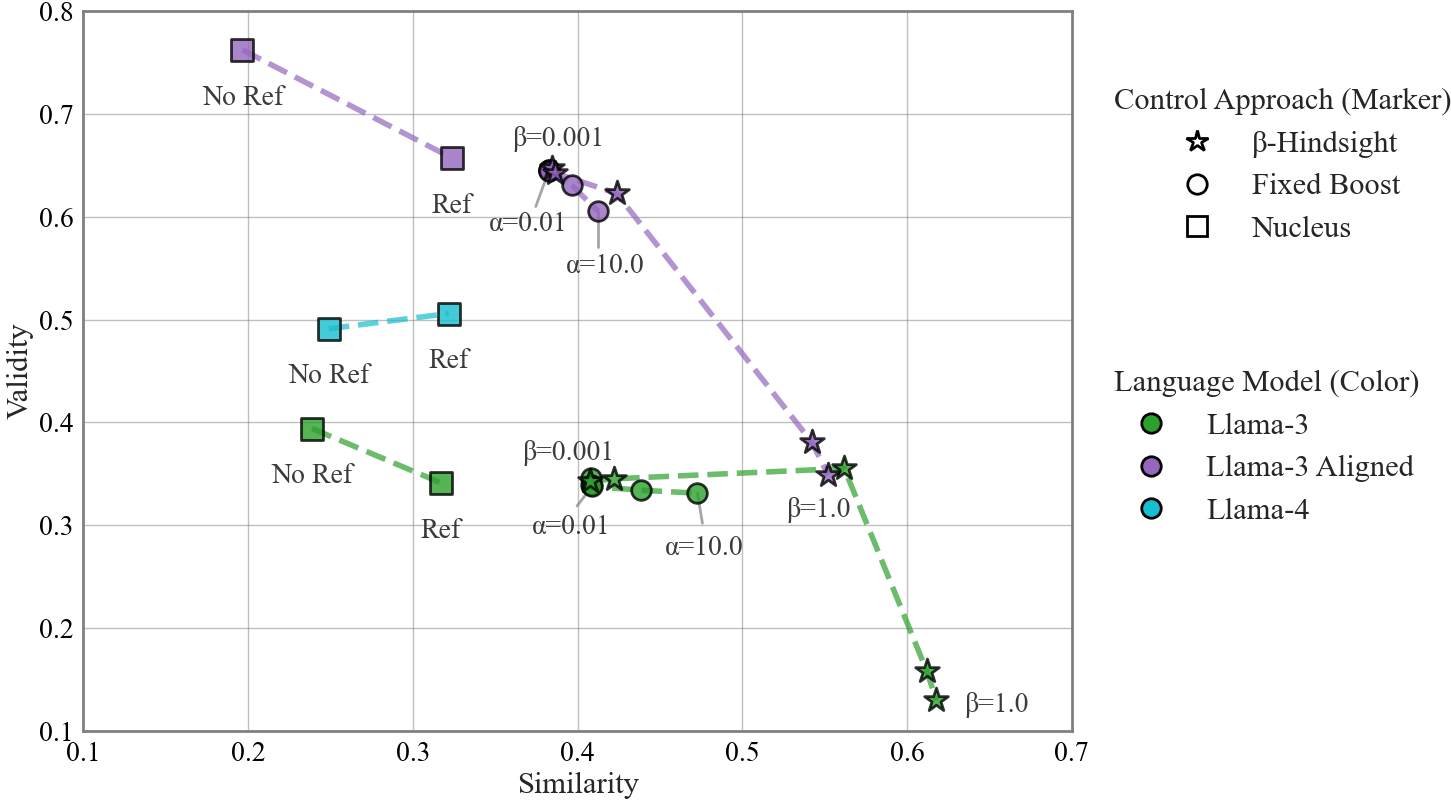
\includegraphics[width=0.99\textwidth]{tradeoff_curve_save_v5.png}
%     \caption{Similarity–validity trade-offs across models (colors) and decoding strategies (shapes). Gumbel Machine combines model alignment (purple) and $\beta$-Hindsight control (star), which yields counterfactuals with higher validity and reference similarity compared to a larger Llama-4 model. $\beta$-Hindsight control traverses a wider-range of the trade-off curve with higher validity compared to Fixed Boost (circle).}
%         \label{fig:tradeoff-curves}
% \end{figure*}


\section{Results, Analysis, Discussion}

We now detail experimental results and perform both human evaluation and ablation studies to verify the effectiveness of our approach. 

% Across all experimental settings, we report our $\beta$-Hindsight sampling approach (Ours) to standard categorical random sampling (Baseline).  In all cases, we instruct the LLM to adhere to the factual student summary while generating a counterfactual response. To induce a counterfactual from the LLM, we instruct the model to form an output for a different expected score by simply changing a single character of the prompt corresponding to the desired score value $z'$. We provide further details on exact model prompts and training details in the Appendix TODO.

% May need to explain these things as well, depending on how results are presented.
% \begin{itemize}
%     \item Ref vs No Ref
%     \item Gumbel Value
%     \item Exact sampling setup (stubbed in comment)
%     \item Llama-4 baseline prompting (baseline)
% \end{itemize}





% \begin{table}[h!t]
% \centering
% \setlength{\tabcolsep}{4pt}
% \scalebox{.9}{
% \begin{tabular}{ll  cc  cc}
% \toprule
% & & \multicolumn{2}{c}{\textbf{CLASSE}} & \multicolumn{2}{c}{\textbf{DREsS}} \\
% \cmidrule(lr){3-4} \cmidrule(lr){5-6}
% \multirow{-2}{*}{\textbf{Model}} & \multirow{-2}{*}{\textbf{Method}} & $\text{Similarity}^\uparrow$ & $\text{Validity}^\uparrow$ & $\text{Similarity}^\uparrow$ & $\text{Validity}^\uparrow$ \\
% \midrule
% \multirow{3}{*}{Haiku}
%   & ME %Minimal-Edit
%     & $0.280\std{0.009}$ & $0.144\std{0.141}$
%     & $0.312\std{0.023}$ & $0.093\std{0.037}$ \\
%   & ICL
%     & $0.281\std{0.011}$ & $0.312\std{0.190}$
%     & $0.314\std{0.012}$ & $0.125\std{0.039}$ \\
%   & I\&R %Identify-and-Replace
%     & $0.451\std{0.044}$ & $0.388\std{0.187}$
%     & $0.384\std{0.066}$ & $\underline{0.441}\std{0.195}$ \\
% \midrule
% \multirow{3}{*}{Sonnet}
%   & ME %Minimal-Edit
%     & $0.376\std{0.043}$ & $0.344\std{0.260}$
%     & $0.375\std{0.051}$ & $0.439\std{0.094}$ \\
%   & ICL
%     & $0.359\std{0.024}$ & $\underline{0.604}\std{0.153}$
%     & $0.418\std{0.073}$ & $\textbf{0.484}\std{0.088}$ \\
%   & I\&R %Identify-and-Replace
%     & $\underline{0.554}\std{0.055}$ & $0.434\std{0.206}$
%     & $\underline{0.477}\std{0.081}$ & $0.405\std{0.179}$ \\
% \midrule
% \multirow{1}{*}{Llama}
%  & GM (Ours)
%     & $0.391\std{0.047}$ & $\textbf{0.668}\std{0.210}$
%     & $\underline{0.477}\std{0.137}$ & $0.404\std{0.084}$ \\
%   % & GM ($\beta{=}0.05$)
%   %   & -- & --
%   %   & $0.477 \pm 0.137$ & $0.404 \pm 0.084$ \\
%   % & GM ($\beta{=}0.10$)
%   %   & $0.391 \pm 0.047$ & $\textbf{0.668} \pm 0.210$
%   %   & $0.493 \pm 0.147$ & $0.395 \pm 0.102$ \\
%   % & GM ($\beta{=}0.25$)
%   %   & $0.444 \pm 0.047$ & $0.595 \pm 0.221$
%   %   & -- & -- \\
%   % & GM ($\beta{=}0.50$)
%   %   & $0.506 \pm 0.057$ & $0.423 \pm 0.302$
%   %   & -- & -- \\
% \midrule
% \multirow{1}{*}{Qwen}
%   & GM (Ours)
%     & $\textbf{0.575}\std{0.092}$ & $0.566\std{0.185}$
%     & $\textbf{0.593}\std{0.092}$ & $0.315\std{0.129}$ \\
%   % & GM ($\beta{=}0.001$)
%   %   & -- & --
%   %   & $0.589 \pm 0.091$ & $0.323 \pm 0.134$ \\
%   % & GM ($\beta{=}0.01$)
%   %   & $0.530 \pm 0.097$ & $0.602 \pm 0.179$
%   %   & $0.589 \pm 0.091$ & $0.322 \pm 0.133$ \\
%   % & GM ($\beta{=}0.05$)
%   %   & $0.550 \pm 0.099$ & $0.588 \pm 0.184$
%   %   & $\underline{0.593} \pm 0.092$ & $0.315 \pm 0.129$ \\
%   % & GM ($\beta{=}0.10$)
%   %   & $\textbf{0.575} \pm 0.092$ & $0.566 \pm 0.185$
%   %   & $\textbf{0.607} \pm 0.098$ & $0.287 \pm 0.112$ \\
% \bottomrule
% \end{tabular}}
% \caption{ Comparing counterfactual LLM approaches across different closed and open-weight models. We observe GM translates across open-weight models and has comparable performance to larger closed-weight models.}
% \label{tab:gm_vs_closed}
% \end{table}



% \begin{table*}[t]
% \centering
% \begin{tabular}{l | cc | cc}
% \toprule
% & \multicolumn{2}{c|}{\textbf{CLASSE}} & \multicolumn{2}{c}{\textbf{DREsS}} \\
% \cmidrule(lr){2-3} \cmidrule(lr){4-5}
% \textbf{Configuration} & Sim ($\uparrow$) & Val ($\uparrow$) & Sim ($\uparrow$) & Val ($\uparrow$) \\
% \midrule
% $\beta$-Hindsight (decoding only)
%     & $0.560 \pm 0.020$ & $0.168 \pm 0.024$
%     & $0.402 \pm 0.048$ & $0.148 \pm 0.067$ \\
% + SFT (no DPO)
%     & $\textbf{0.795} \pm 0.036$ & $-0.026 \pm 0.073$
%     & $\textbf{0.733} \pm 0.053$ & $-0.005 \pm 0.062$ \\
% + SFT + DPO \emph{(full GM)}
%     & $0.391 \pm 0.047$ & $\textbf{0.668} \pm 0.210$
%     & $0.493 \pm 0.147$ & $\textbf{0.395} \pm 0.102$ \\
% \bottomrule
% \end{tabular}
% \caption{Alignment ablation on Llama at $\beta{=}0.10$. Each row adds a stage of the GM pipeline on top of $\beta$-Hindsight decoding: SFT alone collapses validity (rubric-adherence is lost while similarity to the reference is maximized), while adding DPO recovers validity at the cost of some similarity. Best result per column in \textbf{bold}.}
% \label{tab:ablation_alignment}
% \end{table*}

% \begin{table*}[h!t]
% \centering
% \setlength{\tabcolsep}{5pt}
% \begin{tabular}{ccc | cc | cc}
% \toprule
% & & & \multicolumn{2}{c|}{\textbf{CLASSE}} & \multicolumn{2}{c}{\textbf{DREsS}} \\
% \cmidrule(lr){4-5} \cmidrule(lr){6-7}
% \multirow{-2}{*}{\textbf{$\beta$-H}} & \multirow{-2}{*}{\textbf{SFT}} & \multirow{-2}{*}{\textbf{DPO}} & $\text{Similarity}^\uparrow$ & $\text{Validity}^\uparrow$ & $\text{Similarity}^\uparrow$ & $\text{Validity}^\uparrow$ \\
% \midrule
% $-$ & $-$ & $-$
%     & $0.314\std{0.016}$ & $0.183\std{0.062}$
%     & $0.305\std{0.009}$ & $0.188\std{0.119}$ \\
% $-$ & \checkmark & $-$
%     & $0.382\std{0.045}$ & $0.151\std{0.130}$
%     & $0.290\std{0.021}$ & $0.102\std{0.049}$ \\
% $-$ & \checkmark & \checkmark
%     & $0.324\std{0.031}$ & $\textbf{0.688}\std{0.109}$
%     & $0.224\std{0.021}$ & $\textbf{0.608}\std{0.182}$ \\
% \midrule
% \checkmark & $-$ & $-$
%     & $0.560\std{0.020}$ & $0.168\std{0.024}$
%     & $0.402\std{0.048}$ & $0.148\std{0.067}$ \\
% \checkmark & \checkmark & $-$
%     & $\textbf{0.795}\std{0.036}$ & $-0.026\std{0.073}$
%     & $\textbf{0.733}\std{0.053}$ & $-0.005\std{0.062}$ \\
% \checkmark & \checkmark & \checkmark
%     & $0.391\std{0.047}$ & $0.668\std{0.210}$
%     & $0.477\std{0.137}$ & $0.404\std{0.084}$ \\
% \bottomrule
% \end{tabular}
% \caption{Alignment ablation on Llama at $\beta{=}0.10$. Checkmarks indicate which components are active. SFT alone maximizes similarity but collapses validity; DPO recovers validity at the cost of some similarity. The full GM configuration combines all three. Best result per column in \textbf{bold}.}
% \label{tab:ablation_alignment}
% \end{table*}


\subsection{Counterfactual Approach Comparisons}

In Table~\ref{tab:llama_results}, we report the results of our experiments comparing GM to baseline LLM-based counterfactual approaches. In this experiment, we run all settings on Llama-3 and set $\beta=0.1$ and $\beta=0.05$ for CLASSE and DREsS, respectively, based on tuning experiments reported in Section~\ref{sec:tuning}. On CLASSE, we observe that our approach noticeably improves validity across both datasets and yields higher similarity scores. While the I\&R approach shows a higher similarity score than GM, its validity is the lowest among the approaches. This result suggests that I\&R produces counterfactuals that are more similar to the reference but not accurate with respect to the rubric, while the counterfactuals produced by GM are more accurate and similar. On DresS, we observe that GM outperforms all baselines on both metrics, but do not see as large of an improvement on validity. This observation suggests that GM can produce more rubric-aligned counterfactuals when the writing samples are more homogeneous, e.g., for summarization, compared to open-ended writing. 
%This result suggests the GM is an effective counterfactual approach for both shorter summarization tasks and longer open-ended writing, but produces more .



\subsection{Tuning Gumbel Noise Control} \label{sec:tuning}

In Figure~\ref{fig:pareto-front}, we report the results of our experiments to tune the controllable $\beta$ parameter in the GM. In these experiments, we vary the control signal across a range of values for GM and compare with Vocab Bias, a simple decoding strategy that adds a tunable $\alpha$ to all logits for all tokens in the reference summary \cite{yang_fudge_2021}. For GM, we sweep the control parameter $\beta$ across the values $\beta \in \{0.001, 0.1, 0.2, 0.3, 0.4, 1.0\}$ for CLASSE and $\beta \in \{0.05, 0.2, 0.4, 0,5, 0.6, 0.7, 0.8, 1.0\}$ for DREsS. Higher values of $\beta$ emphasize similarity to the original student response, while lower values prioritize satisfying the desired target score. For Vocab Bias, we sweep the control parameter $\alpha$ across the values $\alpha \in \{0.01, 5.0, 10.0\}$ for CLASSE and $\alpha \in \{0.01, 1.0, 5.0\}$ for DREsS. Higher values of $\alpha$ induce stronger similarity to reference tokens. We observe that values outside these ranges result in collapses in model fluency due to excessive logit manipulation.

Comparing the two approaches, we observe that for GM, increasing values of $\beta$ enable a trade-off between similarity that can explore a much wider range of the Pareto front compared to Vocab Bias. Further, we observe that GM tends to maintain higher validity with increasing similarity values. These observations suggest that recovered Gumbel noise provides a more effective control signal for generating similar counterfactual randomness than using token-level heuristics for similarity control. This finding suggests that similarity control in LLMs is more robust when the entire sampling trajectory and random states are considered rather than solely token-level alignment.

\begin{figure*}[t]
        \centering
        \begin{subfigure}{0.49\textwidth}
            \centering
            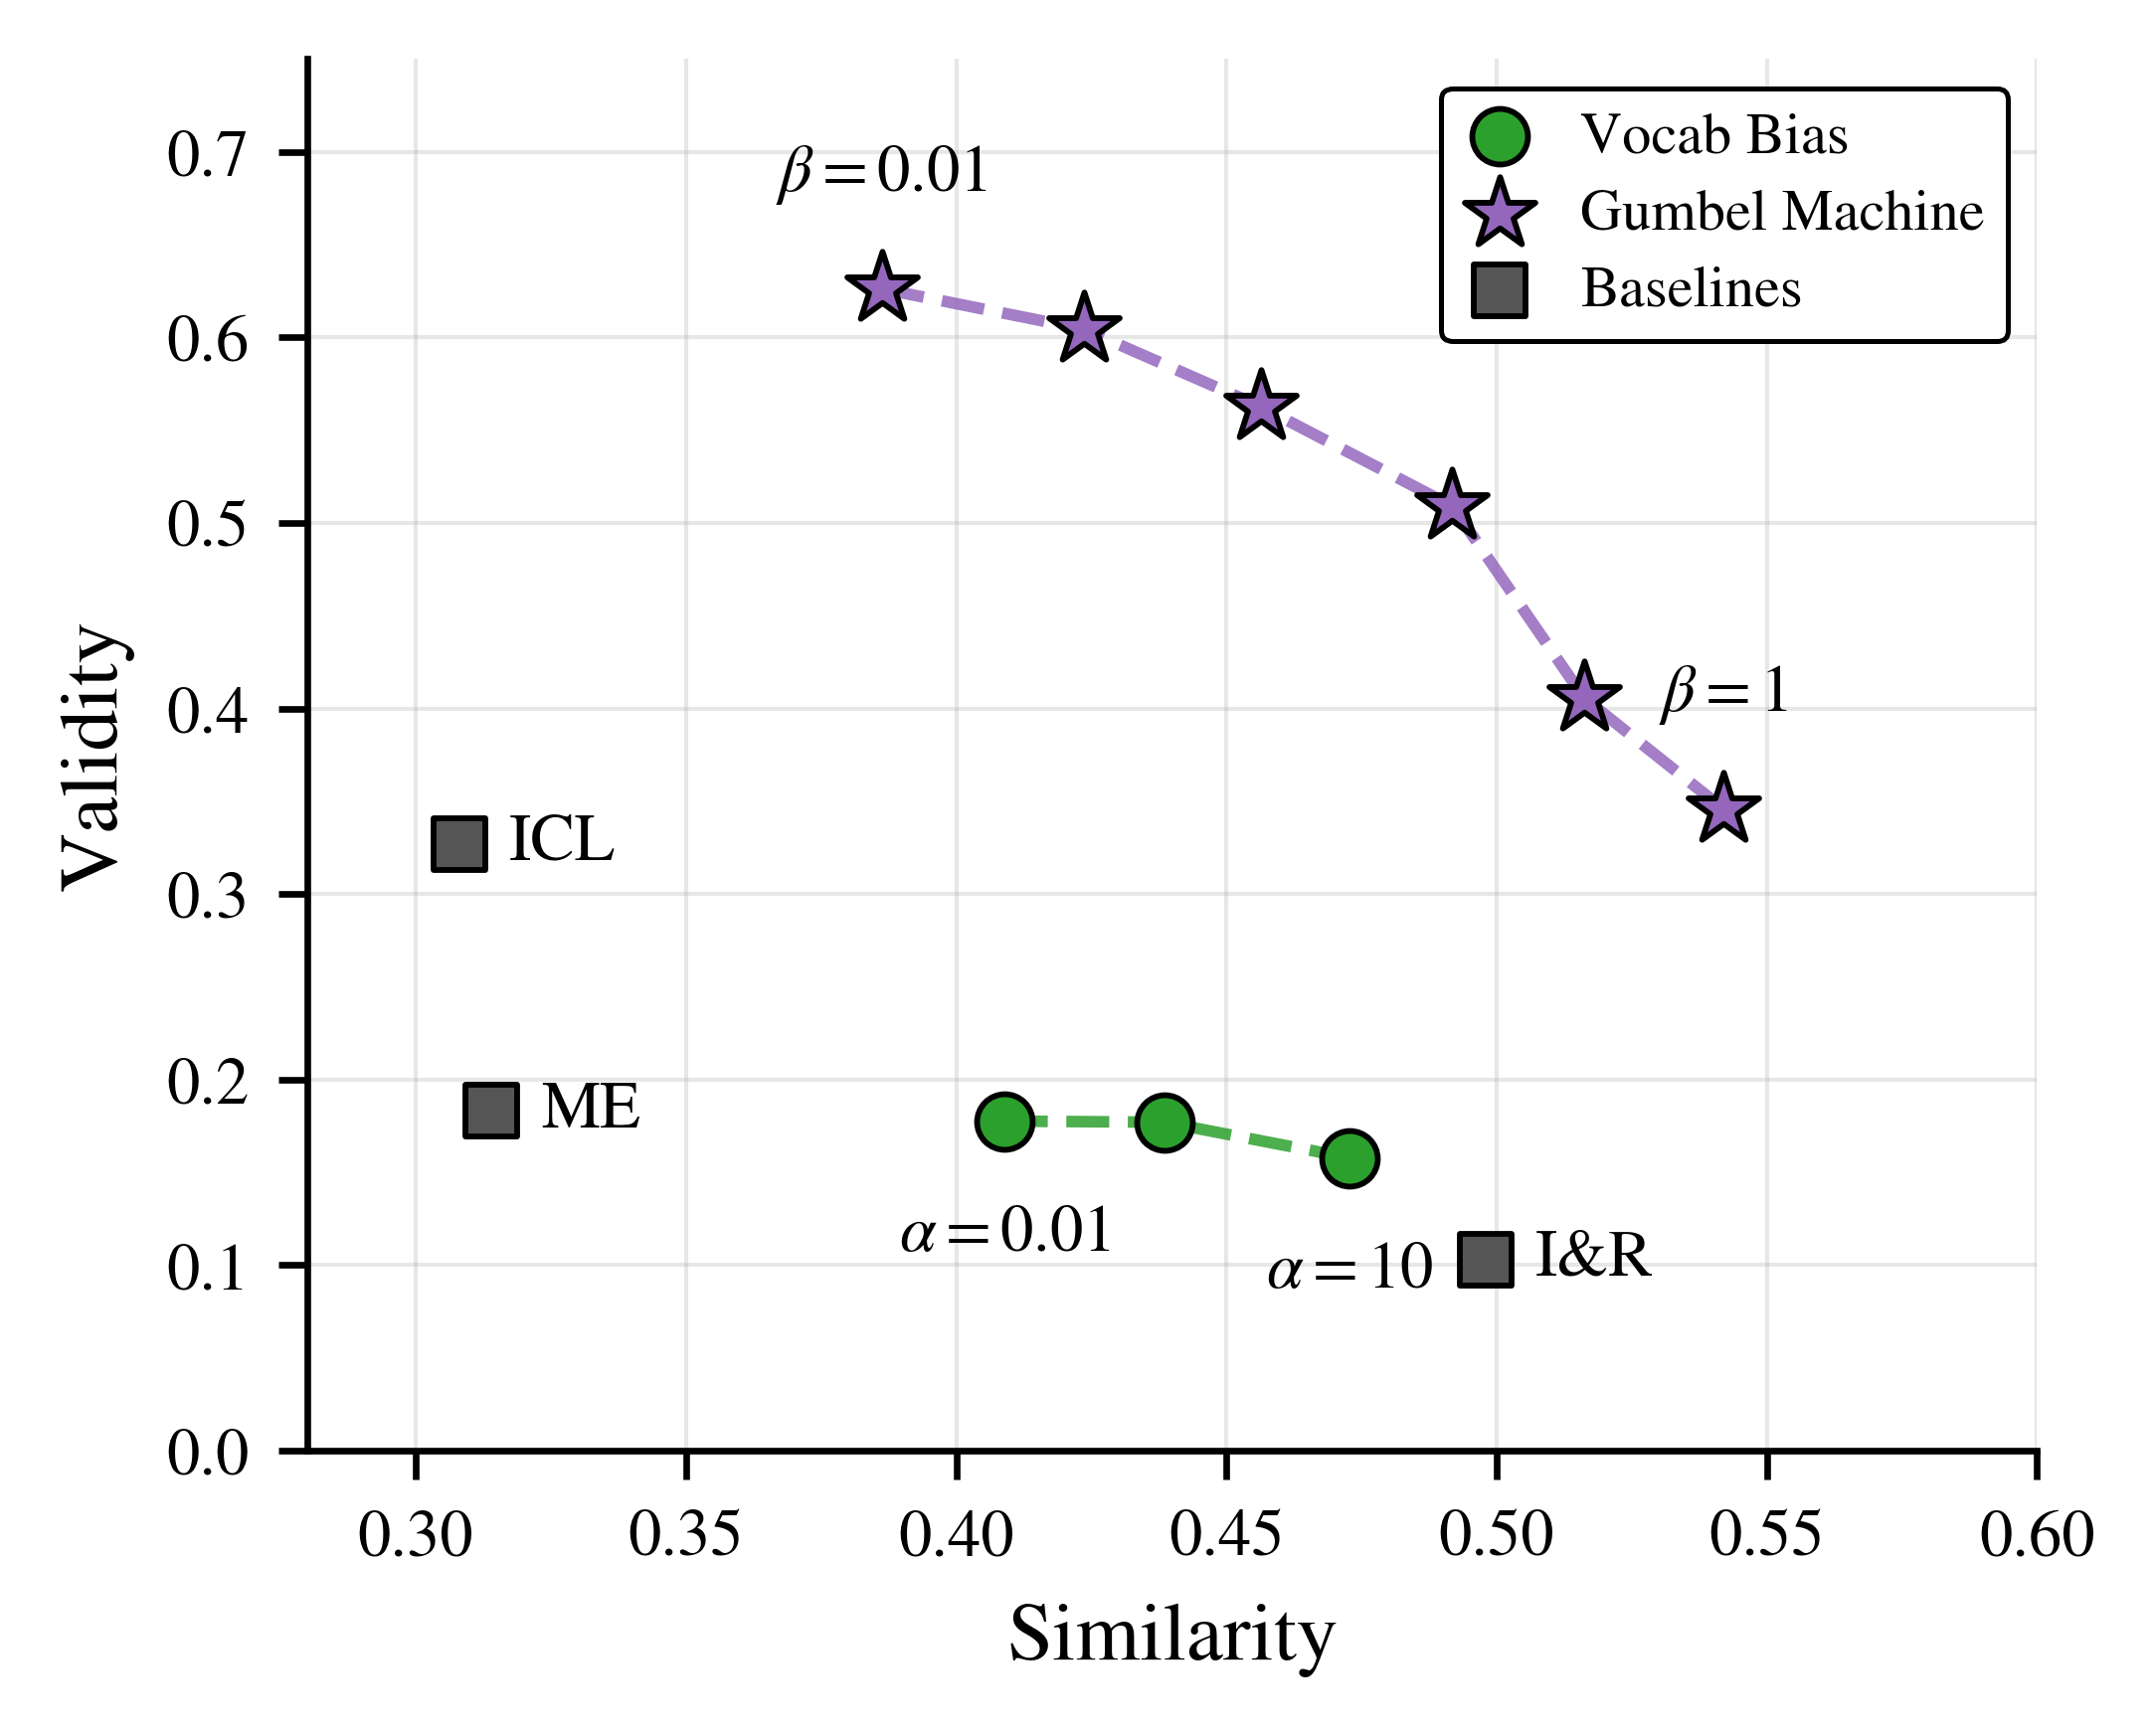
\includegraphics[width=\linewidth]{paper_tradeoff_v4_larger.png}
            \caption{CLASSE}
            \label{fig:pareto-front-classe}
        \end{subfigure}
        \hfill
        \begin{subfigure}{0.49\textwidth}
            \centering
            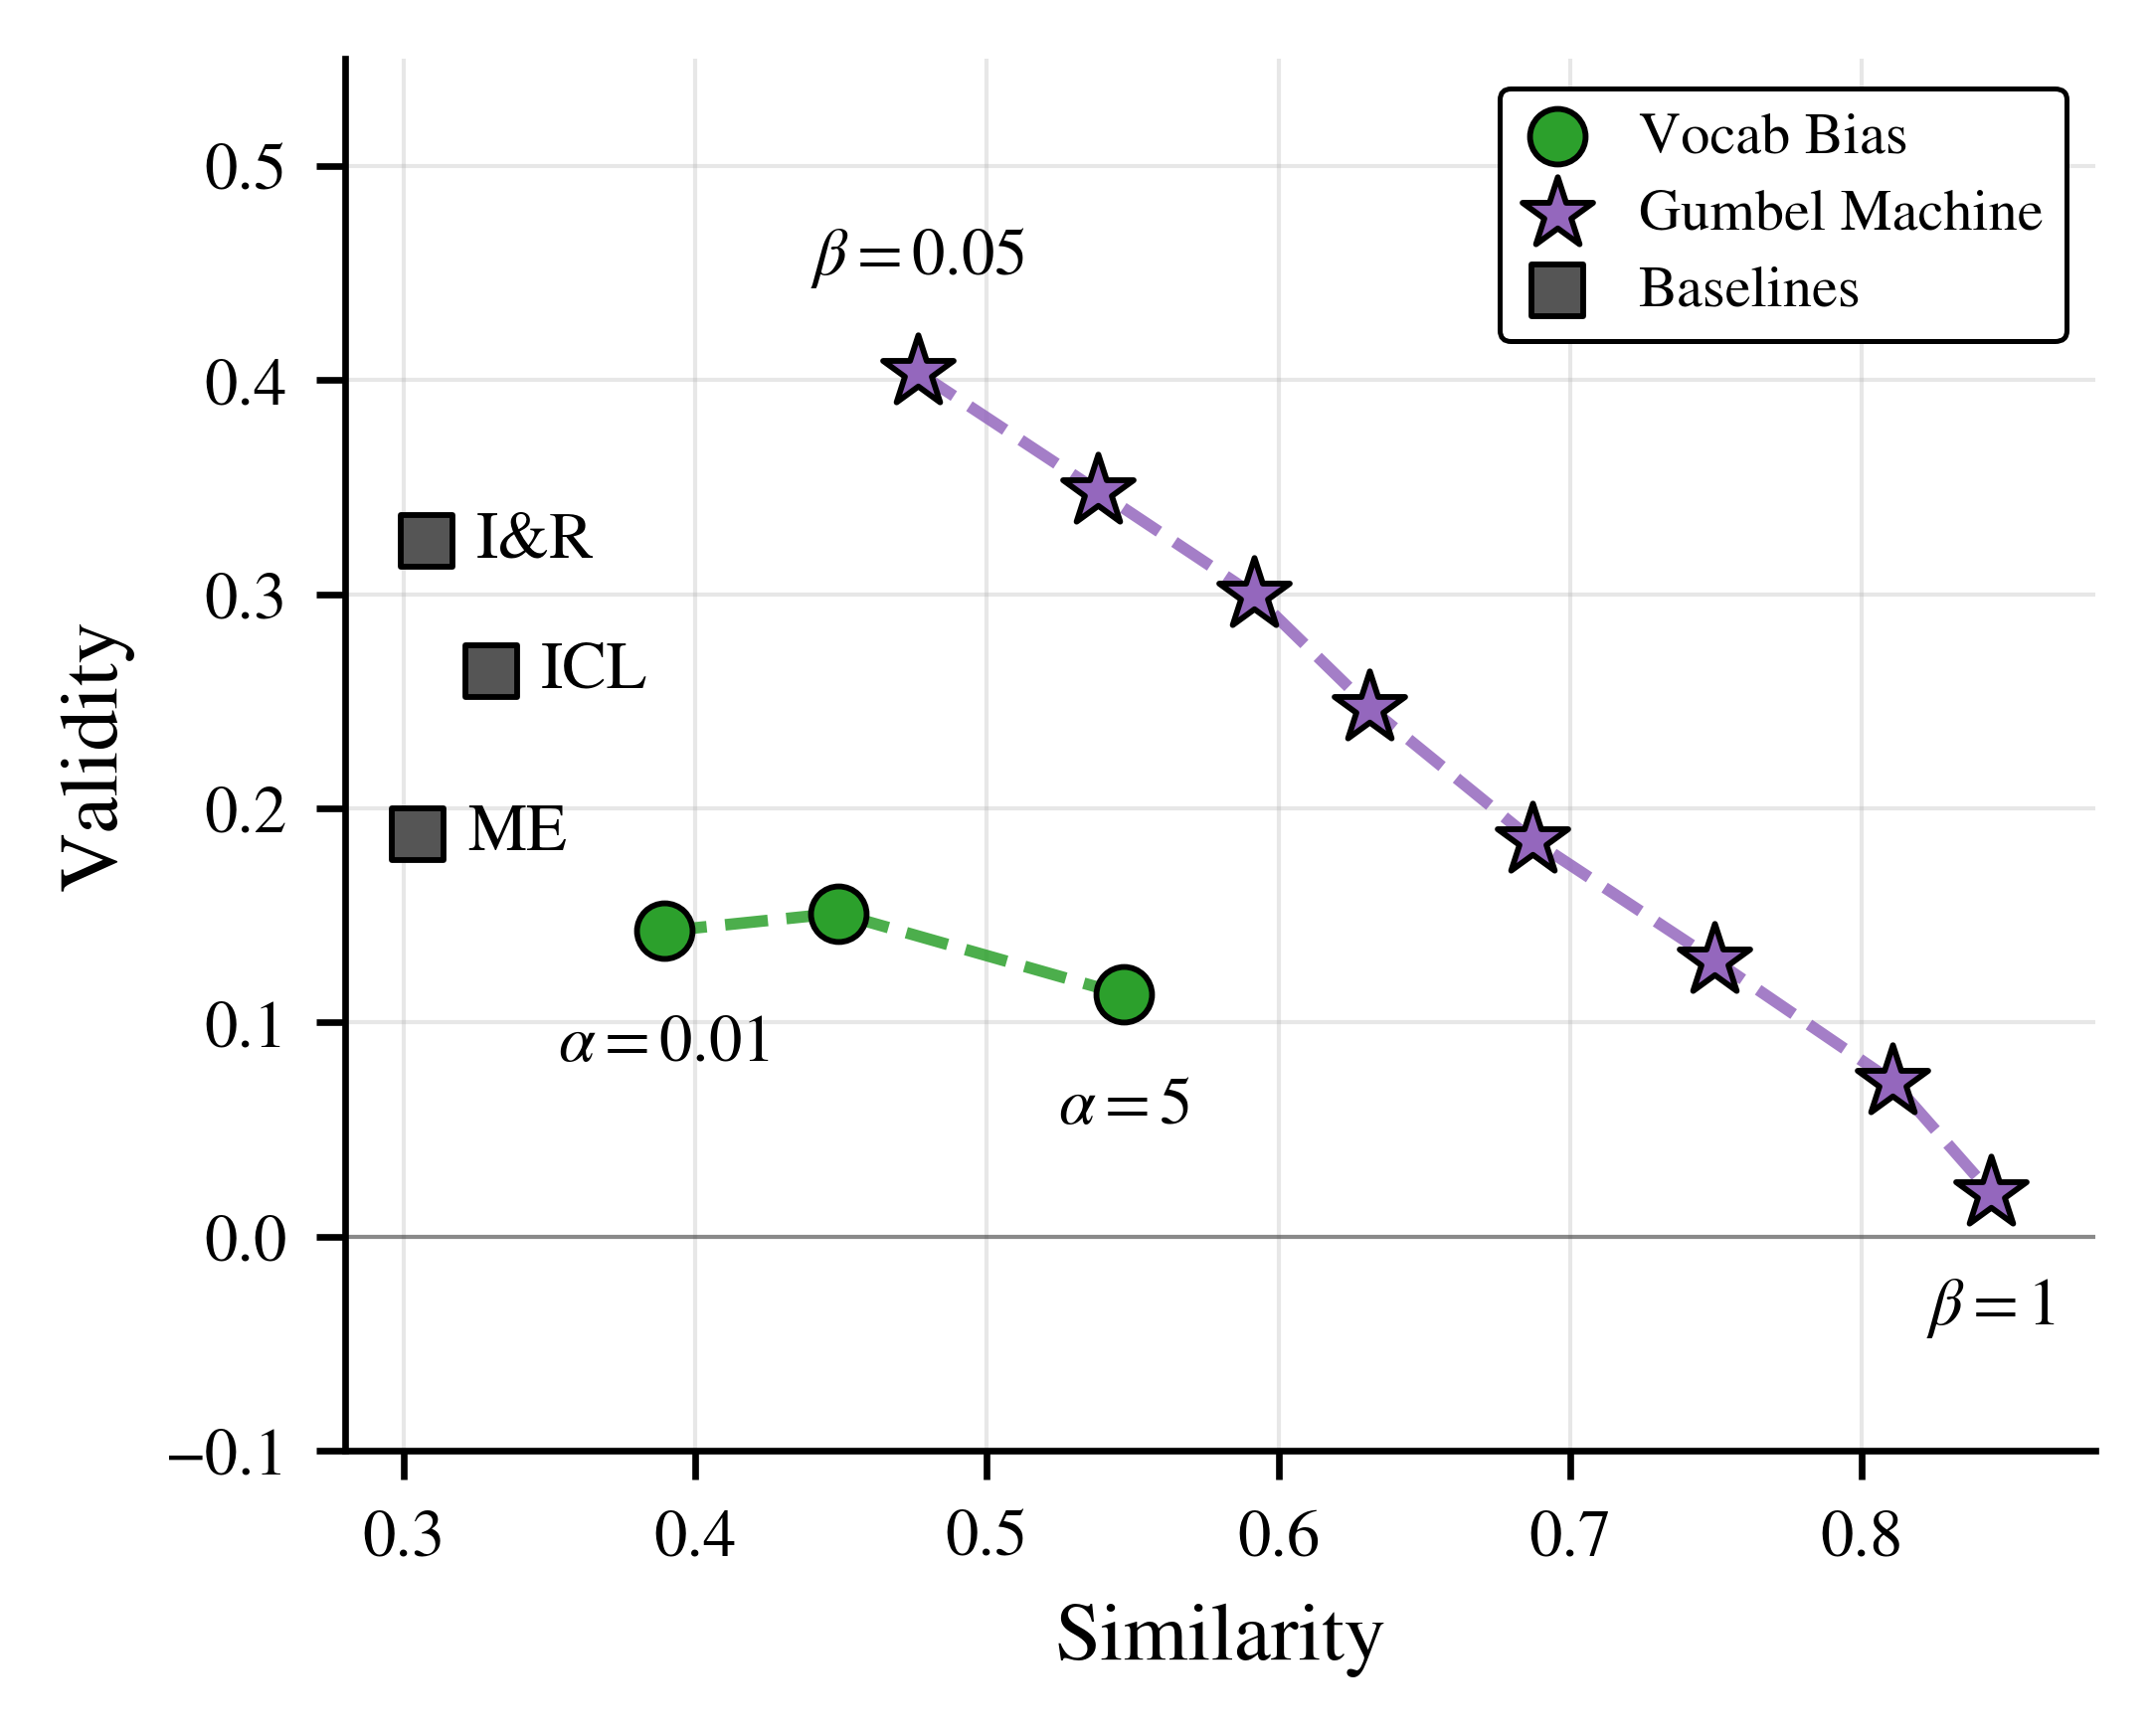
\includegraphics[width=\linewidth]{dress_tradeoff_v1_larger.png}
            \caption{DREsS}
            \label{fig:pareto-front-dress}
        \end{subfigure}
        \caption{Similarity–validity trade-offs comparing Gumbel Machine with a logit bias and baseline approaches (ME - Minimal-Edit, ICL - In-Context Learning, I\&R - Identify-and-Replace) on CLASSE (left) and DREsS (right). Gumbel Machine provides a tunable tradeoff between competing metrics, occupying a different region of the Pareto frontier than the logit-bias baseline.}
        \label{fig:pareto-front}
\end{figure*}

\subsection{Cross-LLM Comparisons}

In Table~\ref{tab:gm_vs_closed}, we report results comparing our approach to other models, Qwen-3 and Claude (prompting-only). 
%For both open-weight models we run our method with the same $\beta$ values of $0.1$ and $0.05$ for CLASSE and DREsS respectively. 
On CLASSE, Llama-3-based GM outperforms the strongest Sonnet-based validity baseline (ICL) on both metrics; Qwen-3-based GM outperforms Sonnet's strongest similarity baseline (Identify-and-Replace) across both metrics. On DREsS, GM improves on similarity compared to proprietary models, but does not reach the same levels of validity in some settings. This result suggests that for longer open-ended writing tasks, the capacity of a larger, more capable base LLM helps. 
%is required to maintain validity over longer time horizons beyond what is possible with training for smaller models. 
Moreover, the result indicates that combining our approach with a larger open-weight model may yield further improvements, but at the expense of higher computational costs. Overall, these results suggest that our GM approach is generalizable across open-weight model families; more importantly, we obtain counterfactuals that are either better than or comparable to those generated by a much larger proprietary model.

\subsection{Human Evaluation}



We conduct an IRB-approved human evaluation study to evaluate the effectiveness of our approach and the quality of the generated counterfactual student writing. We employ four evaluators via Upwork \cite{upwork}, all of whom have experience teaching English in the United States across elementary, middle school, high school levels.

We focus our evaluation on student summaries from the CLASSE dataset, since the shorter, student-written summaries in CLASSE are easier to evaluate at scale than the DREsS essays. We show each evaluator 50 student writing summaries and two counterfactual rewrites of each summary. We then ask them to evaluate each pair of rewritten summaries and compare them across three dimensions: improvement relative to the scoring criterion, similarity to the original summary, and overall pedagogical utility. We select 10 writing samples for each of the 5 criteria and stratify sampling by the original student score on each criterion to ensure that the evaluation includes student writing at different quality levels. We generate rewrites with the targeted score set to the maximum score of 4, sampling from both the GM and the ME baselines. In this setting, both approaches generate rewrites with similar validity, yielding average scores of $3.64/4$ and $3.68/4$, respectively. Therefore, our evaluation setting enables a fair comparison between the two approaches that generate different rewrites but at the same level of validity. To prevent positional bias, we randomize the ordering of rewrites from both approaches.

We report the results of this evaluation in Table~\ref{tab:human_eval}. We observe that evaluators rate GM outputs as more similar to the reference student writing in 62\% of contested cases ($p=0.018$), and give a significantly higher aggregate similarity rating ($p=0.033$). Moreover, our automated similarity metric has moderate yet statistically significant correlation with average teacher similarity ratings ($\rho=0.48$, $p<0.001$). We find no significant difference between the approaches in terms of score improvement (as expected) and utility. However, we observe that when the evaluator judges the GM rewrite as more similar, they also prefer GM on utility in 75\% of contested cases ($\chi^2(4)=57.8$, $p<0.001$). 
% In a per-rating breakdown analysis, we find that GM rewrites are preferred to ME in 92\% of contested cases when the original student work is rated a 3, suggesting that GM performs noticeably better in cases where student rewriting is close to meeting a given criterion but marginally different. 
These results highlight reference similarity as an important factor in creating pedagogically useful feedback for students and demonstrate that fine-grained control techniques beyond prompt design are directionally necessary towards creating automated rewriting feedback systems that are faithful to student writing preferences. We report further details and results of our teacher evaluation in Appendix~\ref{sec:apdx-human-eval}.

 % \ml{this last sentence basically repeats what you wrote in this paragraph and adds nothing new. come up with a deeper discussion?} 



\begin{table}[t]
\small
\centering
\setlength{\tabcolsep}{3pt}
\scalebox{1}{
\begin{tabular}{ccc | cc | cc}
\toprule
& & & \multicolumn{2}{c|}{\textbf{CLASSE}} & \multicolumn{2}{c}{\textbf{DREsS}} \\
\cmidrule(lr){4-5} \cmidrule(lr){6-7}
\multirow{-2}{*}{\textbf{$\beta$-Hindsight}} & \multirow{-2}{*}{\textbf{SFT}} & \multirow{-2}{*}{\textbf{DPO}} & $\text{Sim}^\uparrow$ & $\text{Val}^\uparrow$ & $\text{Sim}^\uparrow$ & $\text{Val}^\uparrow$ \\
\midrule
$-$ & $-$ & $-$
    & $0.314$ & $0.183$
    & $0.305$ & $0.188$ \\
$-$ & \checkmark & $-$
    & $0.382$ & $0.151$
    & $0.290$ & $0.102$ \\
$-$ & \checkmark & \checkmark
    & $0.324$ & $\textbf{0.688}$
    & $0.224$ & $\textbf{0.608}$ \\
\midrule
\checkmark & $-$ & $-$
    & $\underline{0.560}$ & $0.168$
    & $0.402$ & $0.148$ \\
\checkmark & \checkmark & $-$
    & $\textbf{0.795}$ & $\text{-}0.026$
    & $\textbf{0.733}$ & $\text{-}0.005$ \\
\checkmark & \checkmark & \checkmark
    & $0.391$ & $\underline{0.668}$
    & $\underline{0.477}$ & $\underline{0.404}$ \\
\bottomrule
\end{tabular}}
\caption{Ablation study on the components of GM. We observe that SFT alone drastically improves similarity at the cost of validity and that DPO is necessary to realize counterfactual results that balance both axes.}
\label{tab:ablation_alignment}
\end{table}

\subsection{Ablation Studies}\label{sec:foresight}
% \subsection{Foresight Enhances Hindsight Control}

In Table~\ref{tab:ablation_alignment}, we report the results of an ablation on the training and logit control components of GM, running each configuration on Llama-3. We observe a distinctive trend in the introduction of each component. With $\beta$-Hindsight decoding alone and no training, we observe improved similarity at marginally lower validity. This result suggests that recovered Gumbel noise can steer the sampling trajectory toward the reference but does not induce rubric-adherent counterfactuals. Training the model with SFT on student writing amplifies the noise's control influence, resulting in a large jump in similarity while validity collapses to near zero. This result suggests that SFT is necessary to adapt a model to student writing style, which may not be statistically likely for a pre-trained model. 
%This collapse suggests an increased model sensitivity to the Gumbel noise control, and could be explained that the model has a strong preference to vocabularly and word sequences that are frequent in the trained student writing samples. 
Notably, adding DPO after SFT significantly improves the model's capability on this task. This result suggests that by contrasting generations with different scores, DPO helps the LLM with controllable generation, while $\beta$-Hindsight remains key to maintaining similarity to original student writing, which prompting alone cannot achieve. All three components are therefore necessary to produce valid counterfactuals that are similar to the reference. We report the results of an additional ablation study on the prompt configuration in Appendix~\ref{apx:prompt-ablate}. 

% only encodes the likelihood of a simple instruction-following process with high precision

% must capture not only information needed to produce the style but also the information needed to  needs to capture this stylistic control but also the random c

% in an unlikely  without also needing to encode the randomness of the system to produce the exact token configuration observed in the output. 

% These findings may be somewhat surprising since it suggests a signal with weaker information has a stronger control influence. Intuitively, the in-context tokens should bias the logits of the reference tokens, resulting in recovered noise values with lower magnitude and higher entropy. Therefore, we would expect the resulting logit influence to be smaller and less observable control. However, these results suggest the opposite, that a more subtle signal has a noticeably stronger control influence, at least in this setting. We leave further investigation into these interactions as future work.

% We would expect that the recovered noise values with reference inclusion would have higher lower information (higher entropy), since, intuitively, the in-context tokens should bias the resulting logits to be higher during recovery. However, this high entropy noise appears to encode information about the generative trajectory and enforce the model to adhere to a random state, which would result in the echoed reference summary. This biasing then appears to cause the model to adhere more strongly to this trajectory on replay. 
% In the other hand, we'd expect low entropy noise in a in an excluded-reference setting which should have a stronger impact on the model output. However, the resulting influence appears to be weaker in enforcing similarity, with less observed influence on similarity despite
% having expectantlydoes not appear to have as strong of an influence on controlling for random noise, suggesting that the noise may be also accounting for 

% the recovered noise values without a reference have an entropy that is too strong

% that reference inclusion a necessary condition for effective $\beta$-Hindsight control. This result is perhaps surprising, since intuitively we would expect that including a reference would result in recovered noise that has lower information about the stochastic state, and 


% One possible explanation for this finding is that including the reference results in recovered noise that has lower entropy  of the noise recovered while including the reference contains more information during surprising events, resulting in lower entropy and that causes increased control. 

% This finding suggests that recovered noise implicitly encodes aspects of the generative trajectory induced by the original input, rather than functioning as an independent source of randomness. \mh{TODO think about this a bit more and add 1-2 implication/interpretation sentences}

% \subsection{Inspecting the Gumbel Noise}

% \mh{If I have space/time, here, I plan to investigate the gumbel values across settings where the noise is effective and ineffective. Goal for the analysis would be to get some mechanistic understanding of why the noise works and why Foresight is critical. For example difference between ref/no ref or base models/trained models. I could look at descriptive statistics on measures such as overall magnitude or the values of the bounds.  Maybe this could be rolled into sec 5.2}

% Importance of training, tradeoff curve b/w perf and similarity with $\beta$ regularization

% \subsection{Discussion}

% which, in practice, is more  than simply computing the observed logit maximum. Second, their replay procedure does not include $\beta$ regularization on replay, as their work is more theoretical in nature and not focused on using Gumbel noise for a downstream task.
% \mh{Not sure exactly where the last paragraph belongs, maybe a footnote?} \al{I think it's okay here, but it's definitely worth saying these things. Related work would also be a reasonable place.}

% We owe it all to sample citation\cite{Ando2005}.

\section{Conclusions and Future Work}
% Synthesize the paper, how all the pieces fit together to make your point
% What we did in 1 sentence
We present the Gumbel Machine, a modular approach to counterfactual generation that leverages preference alignment and replayed random state with $\beta$-Hindsight control.
% How it works in a sentence, key components
% We introduce $\beta$-Hindsight control, an inference-time control that utilizes recovered Gumbel noise to induce similarity and enhance model rubric-adherence through a preference optimization strategy that is inherently compatible with ordinal data. 
% How we create out evidence to evaluate what we propose as contributions + key observations
We evaluate our approach on two datasets of student-written summaries and demonstrate that it effectively generates counterfactual student work that is both rubric-valid and similar to the original. This work demonstrates that recovered generative randomness can serve as a tunable control signal with immediate application.
% Overall, this work reframes generative randomness as a controllable resource, demonstrating how recovered stochastic state can be leveraged as a practical and extensible control signal for language generation.

% Then outline future work, space permitting
Our work outlines future directions that include: evaluating this approach across other domains and generation tasks, assessing the pedagogical effectiveness of generated counterfactuals relative to conventional writing feedback, and further investigation into the necessary and sufficient conditions for recovering noise that is effective for control.


\clearpage
% \section*{Acknowledgments}

% Bibliography entries for the entire Anthology, followed by custom entries
%\bibliography{anthology,custom}
% Custom bibliography entries only
% AAAI permits \small (9pt) references when over length; keeps them to 2 pages.
{\small
\bibliography{custom}
}

\end{document}
